\documentclass{vkr}
\usepackage[english, russian]{babel} % переносы
\usepackage{graphicx} % для вставки картинок
\graphicspath{{images/}} % путь к изображениям
\usepackage[hidelinks]{hyperref}
\usepackage{float} % определяет метод H для рисунка с переносом на следующую страницу, ели не помещается
\usepackage{pdflscape}
\addto{\captionsrussian}{\renewcommand{\refname}{СПИСОК ИСПОЛЬЗОВАННЫХ ИСТОЧНИКОВ}}
\usepackage{xltabular} % для вставки таблиц
\usepackage{makecell}
\renewcommand\theadfont{} % шрифт в /thead
\usepackage{array} % для определения новых типов столбцов таблиц
\newcolumntype{T}{>{\centering\arraybackslash}X} % новый тип столбца T - автоматическая ширина столбца с выравниванием по центру
\newcolumntype{R}{>{\raggedleft\arraybackslash}X} % новый тип столбца R - автоматическая ширина столбца с выравниванием по правому краю
\newcolumntype{C}[1]{>{\centering\let\newline\\\arraybackslash\hspace{0pt}}m{#1}} % новый тип столбца C - фиксированная ширина столбца с выравниванием по центру
\newcolumntype{r}[1]{>{\raggedleft\arraybackslash}p{#1}} % новый тип столбца r - фиксированная ширина столбца с выравниванием по правому краю
\newcommand{\centrow}{\centering\arraybackslash} % командой \centrow можно центрировать одну ячейку (заголовок) в столбце типа X или p, оставив в оcтальных ячейках другой тип выравнивания
\newcommand{\finishhead}{\endhead\hline\endlastfoot}
\newcommand{\continuecaption}[1]{\caption*{#1}\\ \hline }
\usepackage{etoolbox}
\AtBeginEnvironment{xltabular}{\refstepcounter{tablecnt}} % подсчет таблиц xltabular, обычные таблицы подсчитываются в классе

\usepackage[tableposition=top]{caption} % подпись таблицы вверху
\captionsetup{strut=off}
\setlength{\intextsep}{0pt} % Vertical space above & below [h] floats
\setlength{\textfloatsep}{0pt} % Vertical space below (above) [t] ([b]) floats
\DeclareCaptionLabelFormat{gostfigure}{Рисунок #2} %подпись рисунка
\DeclareCaptionLabelFormat{gosttable}{Таблица #2} %подпись таблицы
\DeclareCaptionLabelSeparator{gost}{~--~} %разделитель в рисунках и таблицах
\captionsetup{labelsep=gost}
\captionsetup[figure]{aboveskip=10pt,belowskip=4mm,justification=centering,labelformat=gostfigure} % настройка подписи рисунка
\captionsetup[table]{font={stretch=1.41},skip=0pt,belowskip=0pt,aboveskip=8.5pt,singlelinecheck=off,labelformat=gosttable} % настройка подписи таблицы

\usepackage{amsmath}

\setlength{\LTpre}{8mm} % отступ сверху таблицы
\setlength{\LTpost}{6mm} % отступ снизу таблицы

\usepackage{enumitem}
\setlist{nolistsep,wide=\parindent,itemindent=*} % отступы вокруг списков, выравнивание с учетом разделителя

\usepackage{color} %% это для отображения цвета в коде
\usepackage{listings} %% листинги кода
\setmonofont[Scale=0.7]{Verdana} % моноширный шрифт для листинга

\definecolor{codegreen}{rgb}{0,0.6,0}
\definecolor{codegray}{rgb}{0.5,0.5,0.5}
\definecolor{codepurple}{rgb}{0.58,0,0.82}

\lstset{ %
language=C,                 % выбор языка для подсветки (здесь это С)
numbers=left,               % где поставить нумерацию строк (слева\справа)
numberstyle=\tiny,           % размер шрифта для номеров строк
stepnumber=1,                   % размер шага между двумя номерами строк
numbersep=5pt,                % как далеко отстоят номера строк от подсвечиваемого кода
commentstyle=\color{codegreen},
keywordstyle=\color{magenta},
numberstyle=\tiny\color{codegray},
stringstyle=\color{codepurple},
basicstyle=\linespread{0.95}\ttfamily,
backgroundcolor=\color{white}, % цвет фона подсветки - используем \usepackage{color}
showspaces=false,            % показывать или нет пробелы специальными отступами
showstringspaces=false,      % показывать или нет пробелы в строках
showtabs=false,             % показывать или нет табуляцию в строках
frame=single,              % рисовать рамку вокруг кода
tabsize=2,                 % размер табуляции по умолчанию равен 2 пробелам
captionpos=t,              % позиция заголовка вверху [t] или внизу [b] 
breaklines=true,           % автоматически переносить строки (да\нет)
breakatwhitespace=false, % переносить строки только если есть пробел
escapeinside={\%*}{*)}   % если нужно добавить комментарии в коде
}

\makeatletter % чтобы допускались русские комментарии в листингах
\lst@InputCatcodes
\def\lst@DefEC{%
 \lst@CCECUse \lst@ProcessLetter
  ^^80^^81^^82^^83^^84^^85^^86^^87^^88^^89^^8a^^8b^^8c^^8d^^8e^^8f%
  ^^90^^91^^92^^93^^94^^95^^96^^97^^98^^99^^9a^^9b^^9c^^9d^^9e^^9f%
  ^^a0^^a1^^a2^^a3^^a4^^a5^^a6^^a7^^a8^^a9^^aa^^ab^^ac^^ad^^ae^^af%
  ^^b0^^b1^^b2^^b3^^b4^^b5^^b6^^b7^^b8^^b9^^ba^^bb^^bc^^bd^^be^^bf%
  ^^c0^^c1^^c2^^c3^^c4^^c5^^c6^^c7^^c8^^c9^^ca^^cb^^cc^^cd^^ce^^cf%
  ^^d0^^d1^^d2^^d3^^d4^^d5^^d6^^d7^^d8^^d9^^da^^db^^dc^^dd^^de^^df%
  ^^e0^^e1^^e2^^e3^^e4^^e5^^e6^^e7^^e8^^e9^^ea^^eb^^ec^^ed^^ee^^ef%
  ^^f0^^f1^^f2^^f3^^f4^^f5^^f6^^f7^^f8^^f9^^fa^^fb^^fc^^fd^^fe^^ff%
  ^^^^20ac^^^^0153^^^^0152%
  % Basic Cyrillic alphabet coverage
  ^^^^0410^^^^0411^^^^0412^^^^0413^^^^0414^^^^0415^^^^0416^^^^0417%
  ^^^^0418^^^^0419^^^^041a^^^^041b^^^^041c^^^^041d^^^^041e^^^^041f%
  ^^^^0420^^^^0421^^^^0422^^^^0423^^^^0424^^^^0425^^^^0426^^^^0427%
  ^^^^0428^^^^0429^^^^042a^^^^042b^^^^042c^^^^042d^^^^042e^^^^042f%
  ^^^^0430^^^^0431^^^^0432^^^^0433^^^^0434^^^^0435^^^^0436^^^^0437%
  ^^^^0438^^^^0439^^^^043a^^^^043b^^^^043c^^^^043d^^^^043e^^^^043f%
  ^^^^0440^^^^0441^^^^0442^^^^0443^^^^0444^^^^0445^^^^0446^^^^0447%
  ^^^^0448^^^^0449^^^^044a^^^^044b^^^^044c^^^^044d^^^^044e^^^^044f%
  ^^^^0401^^^^0451%
  %%%
  ^^00}
\lst@RestoreCatcodes
\makeatother


% Режим шаблона (должен быть включен один из трех)
\ВКРtrue
%\Практикаtrue
%\Курсоваяtrue

\newcommand{\Дисциплина}{<<Проектирование и архитектура программных систем>>} % для курсовой
\newcommand{\КодСпециальности}{09.03.04} % Курсовая
\newcommand{\Специальность}{Программная инженерия} % Курсовая
\newcommand{\Тема}{Программная система визуализации трехмерных данных,} % ВКР Курсовая
\newcommand{\ТемаВтораяСтрока}{использующая библиотеку OpenGL}
\newcommand{\ГдеПроводитсяПрактика}{ООО «МЦОБ. Онлайн-сервисы»} % для практики
\newcommand{\РуководительПрактПредпр}{} % для практики
\newcommand{\ДолжнРуководительПрактПредпр}{} % для практики
\newcommand{\РуководительПрактУнивер}{Чаплыгин А. А.} % для практики
\newcommand{\ДолжнРуководительПрактУнивер}{к.т.н. доцент} % для практики
\newcommand{\Автор}{Н.И. Снатенков}
\newcommand{\АвторРод}{Снатенкова Н.И.}
\newcommand{\АвторПолностьюРод}{Снатенкова Николая Ивановича} % для практики
\newcommand{\Шифр}{20-06-0086}
\newcommand{\Курс}{4} % для практики
\newcommand{\Группа}{ПО-02б}
\newcommand{\Руководитель}{В. В. Серебровский} % для ВКР и курсовой
\newcommand{\Нормоконтроль}{А. А. Чаплыгин} % для ВКР
\newcommand{\ЗавКаф}{А. В. Малышев} % для ВКР
\newcommand{\ДатаПриказа}{«04» апреля 2024~г.} % для ВКР
\newcommand{\НомерПриказа}{1616-с} % для ВКР
\newcommand{\СрокПредоставления}{«11» июня 2024~г.} % для ВКР, курсового

\begin{document}
\maketitle
\ifПрактика{}\else{
   \newpage
\begin{center}
\large\textbf{Минобрнауки России}

\large\textbf{Юго-Западный государственный университет}
\vskip 1em
\normalsize{Кафедра программной инженерии}
\vskip 1em
\ifВКР{
        \begin{flushright}
        \begin{tabular}{p{.4\textwidth}}
        \centrow УТВЕРЖДАЮ: \\
        \centrow Заведующий кафедрой \\
        \hrulefill \\
        \setarstrut{\footnotesize}
        \centrow\footnotesize{(подпись, инициалы, фамилия)}\\
        \restorearstrut
        «\underline{\hspace{1cm}}»
        \underline{\hspace{3cm}}
        20\underline{\hspace{1cm}} г.\\
        \end{tabular}
        \end{flushright}
        }\fi
\end{center}
\vspace{1em}
  \begin{center}
  \large
\ifВКР{
ЗАДАНИЕ НА ВЫПУСКНУЮ КВАЛИФИКАЦИОННУЮ РАБОТУ
  ПО ПРОГРАММЕ БАКАЛАВРИАТА}
  \else
ЗАДАНИЕ НА КУРСОВУЮ РАБОТУ (ПРОЕКТ)
\fi
\normalsize
  \end{center}
\vspace{1em}
{\parindent0pt
  Студента \АвторРод, шифр\ \Шифр, группа \Группа
  
1. Тема «\Тема\ \ТемаВтораяСтрока»
\ifВКР{
утверждена приказом ректора ЮЗГУ от \ДатаПриказа\ № \НомерПриказа
}\fi.

2. Срок предоставления работы к защите \СрокПредоставления

3. Исходные данные для создания программной системы:

3.1. Перечень решаемых задач:}

\renewcommand\labelenumi{\theenumi)}

\begin{enumerate}
\item изучить основы и принципы работы библиотеки OpenGL;
\item разработать концептуальную модель графического движка на основе библиотеки OpenGL;
\item спроектировать программную систему визуализации трёхмерных данных;
\item сконструировать и протестировать программную систему визуализации трёхмерных данных.
\end{enumerate}

{\parindent0pt
  3.2. Входные данные и требуемые результаты для программы:}

\begin{enumerate}
\item Входными данными для программной системы являются: файлы трёхмерных моделей, стандартизированные под классический формат файлов геометрии объектов OBJ, с триангулированными вершинами; файлы изображений текстур.
\item Выходными данными для программной системы являются: файлы данных, содержащие в себе информацию о сохраненных и загруженных файлов в проект; вывод визуализированного изображения трёхмерной виртуальной сцены на экран.
\end{enumerate}

{\parindent0pt

  4. Содержание работы (по разделам):
  
  4.1. Введение
  
  4.1. Анализ предметной области
  
4.2. Техническое задание: основание для разработки, назначение разработки,
требования к программной системе, требования к оформлению документации.

4.3. Технический проект: общие сведения о программной системе, проект
данных программной системы, проектирование архитектуры программной системы, проектирование пользовательского интерфейса программной системы.

4.4. Рабочий проект: спецификация компонентов и классов программной системы, тестирование программной системы, сборка компонентов программной системы.

4.5. Заключение

4.6. Список использованных источников

5. Перечень графического материала:

\списокПлакатов

\vskip 2em
\begin{tabular}{p{6.8cm}C{3.8cm}C{4.8cm}}
Руководитель \ifВКР{ВКР}\else работы (проекта) \fi & \lhrulefill{\fill} & \fillcenter\Руководитель\\
\setarstrut{\footnotesize}
& \footnotesize{(подпись, дата)} & \footnotesize{(инициалы, фамилия)}\\
\restorearstrut
Задание принял к исполнению & \lhrulefill{\fill} & \fillcenter\Автор\\
\setarstrut{\footnotesize}
& \footnotesize{(подпись, дата)} & \footnotesize{(инициалы, фамилия)}\\
\restorearstrut
\end{tabular}
}

\renewcommand\labelenumi{\theenumi.}

   \abstract{РЕФЕРАТ}

Объем работы равен \formbytotal{lastpage}{страниц}{е}{ам}{ам}. Работа содержит \formbytotal{figurecnt}{иллюстраци}{ю}{и}{й}, \formbytotal{tablecnt}{таблиц}{у}{ы}{}, \arabic{bibcount} библиографических источников и \formbytotal{числоПлакатов}{лист}{}{а}{ов} графического материала. Количество приложений – 2. Графический материал представлен в приложении А. Фрагменты исходного кода представлены в приложении Б.

Перечень ключевых слов: коммерческий сайт, Система, CMS, Битрикс, Joomla, аддитивные технологии, 3D-принтеры, услуги, сервисы, информатизация, автоматизация, информационные технологии, веб-форма,  Apache, классы, база данных, средства защиты информации, подсистема, компонент, модуль, сущность, информационный блок, метод, контент-редактор, администратор, пользователь, web-сайт.

Объектом разработки является web-сайт компании,  занимающейся производством 3D-принтеров, выпуском оборудования для создания порошков, разработкой программного обеспечения и организацией центров аддитивного производства.

Целью выпускной квалификационной работы является привлечение клиентов, увеличение заказов, информирование о продукции и услугах путем создания сайта компании.

В процессе создания сайта были выделены основные сущности путем создания информационных блоков, использованы классы и методы модулей, обеспечивающие работу с сущностями предметной области, а также корректную работу web-сайта, разработаны разделы, содержащие информацию о компании, ее деятельности, производимой продукции и услугах, разработан сервис по заказу 3D-деталей.

При разработке сайта использовалась система управления контентом "<1С-Битрикс: Управление сайтом">.

Разработанный сайт был успешно внедрен в компании.

\selectlanguage{english}
\abstract{ABSTRACT}
  
The volume of work is \formbytotal{lastpage}{page}{}{s}{s}. The work contains \formbytotal{figurecnt}{illustration}{}{s}{s}, \formbytotal{tablecnt}{table}{}{s}{s}, \arabic{bibcount} bibliographic sources and \formbytotal{числоПлакатов}{sheet}{}{s}{s} of graphic material. The number of applications is 2. The graphic material is presented in annex A. The layout of the site, including the connection of components, is presented in annex B.

List of keywords: commercial website, System, CMS, Bitrix, Joomla, additive technologies, 3D printers, services, services, informatization, automation, information technology, web form, Apache, classes, database, component, module, entity, information block, method, content editor, administrator, user, web site.

The object of the research is the analysis of information technologies for the development of a production company's website.

The object of the development is the website of a company engaged in the production of 3D printers, the production of equipment for the creation of powders, software development and the organization of additive manufacturing centers.

The purpose of the final qualifying work is to attract customers, increase orders, inform about products and services by creating a company website.

In the process of creating the site, the main entities were identified by creating information blocks, classes and methods of modules were used to ensure work with the entities of the subject area, as well as the correct operation of the website, sections containing information about the company, its activities, products and services were developed, a service for ordering 3D parts was developed.

When developing the site, the content management system <<1C – Bitrix: Site Management>> was used.

The developed website was successfully implemented in the company.
\selectlanguage{russian}
}\fi
\tableofcontents
\section*{ОБОЗНАЧЕНИЯ И СОКРАЩЕНИЯ}

ИС -- информационная система.

ИТ -- информационные технологии. 

КТС -- комплекс технических средств.

ОМТС -- отдел материально-технического снабжения. 

ПО -- программное обеспечение.

РП -- рабочий проект.

ТЗ -- техническое задание.

ТП -- технический проект.

UML (Unified Modelling Language) -- язык графического описания для объектного моделирования в области разработки программного обеспечения.

OBJ -- формат файлов описания геометрии, разработанный в Wavefront Technologies для их анимационного пакета Advanced Visualizer. Формат файла является открытым и был принят другими разработчиками приложений 3D-графики.

3D (от англ. 3-dimensional) графика -- раздел компьютерной графики, посвящённый методам создания изображений или видео путём моделирования объектов в трёх измерениях.

GL (Graphic Library) -- это программная библиотека, предназначенная для оказания помощи в рендеринге компьютерной графики на мониторе.
\ifПрактика{}\else{\section*{ВВЕДЕНИЕ}
\addcontentsline{toc}{section}{ВВЕДЕНИЕ}

Трёхмерная компьютерная графика появилась в 1960-х годах. Первые векторные изображения состояли из множества точек и кривых, заданных математической формулой. Айван Сазерленд и Дэвид Эванс основали первую в мире кафедру компьютерной графики в университете Юты, США. Именно в те времена появилась программа Sketchpad (от англ. «альбом для рисования») — предок всех современных 3D-редакторов.

На первых компьютерах можно было работать только с векторными изображениями. Затем появилась растровая графика, которая позволила изображать объекты в виде сетки пикселей. Кроме сплошных цветов и фигур, начали использовать текстуры и тени, расширились возможности рендеринга — превращения кода в финальные изображения.

Трёхмерные объекты математически представляются в виде множества точек - вершин, и в тоже время они, соединенные отрезками, образуют рёбра фигиры, а множество рёбер на одной плоскости образуют поверхности - грани фигуры. Данный массив точек трансформируется с учётом матрицы перспективы камеры, далее - накладываются текстуры на поверхности граней фигуры - изображения также растягивают и трансформируют с учётом перспективы наклона грани, затем - обрабатывают свет, падающий на модель, путём изменения яркости текстуры граней, в зависимости от источников света, и наконец - добавляют тень, которая отбрасывает данная трёхмерная модель.

3D-движок, рендерер или визуализатор является программной системой графического движка (название произошло от английского graphics engine) — промежуточное программное обеспечение, программный движок, основной задачей которого является визуализация двухмерной и трёхмерной компьютерной графики. Может существовать как отдельный продукт или в составе игрового движка. Может использоваться для визуализации отдельных изображений или компьютерного видео. Графические движки, использующееся в программах по работе с компьютерной графикой обычно называются «рендерерами», «отрисовщиками» или «визуализаторами». Само название «графический движок» используется, как правило, в компьютерных играх.

Основное и важнейшее отличие «игровых» графических движков от неигровых состоит в том, что первые должны обязательно работать в режиме реального времени, тогда как вторые могут тратить по несколько десятков часов на вывод одного изображения. Вторым существенным отличием является то, что начиная приблизительно с 1995-1997 года, графические движки производят визуализацию с помощью графических процессоров, которые установлены на отдельных платах — видеокартах. Программные графические движки используют только центральные процессоры.

Как правило, графические движки не распространяются отдельно от игровых. Единственного графического движка без дополнительных компонентов и инструментария недостаточно для создания игры, поэтому разработчики движков продают лишь игровые движки с полным набором инструментов и компонентов. Однако это правило не относится к свободному программному обеспечению. Энтузиасты создают свободные графические движки и свободно их распространяют. Впоследствии разработчики игр могут объединить свободный графический движок с физическим, звуковым и другими компонентами и создать на основе их полноценный игровой движок.

\emph{Цель настоящей работы} – разработка графического движка - программной системы реализующей визуализацию трёхмерных данных, на основе графической библиотеки OpenGL. Для достижения поставленной цели необходимо решить \emph{следующие задачи:}
\begin{itemize}
\item провести анализ предметной области;
\item разработать концептуальную модель программы;
\item спроектировать программную систему;
\item реализовать программную среду используя графическую библиотеку OpenGL.
\end{itemize}

\emph{Структура и объем работы.} Отчет состоит из введения, 4 разделов основной части, заключения, списка использованных источников, 2 приложений. Текст выпускной квалификационной работы равен \formbytotal{lastpage}{страниц}{е}{ам}{ам}.

\emph{Во введении} сформулирована цель работы, поставлены задачи разработки, описана структура работы, приведено краткое содержание каждого из разделов.

\emph{В первом разделе} на стадии описания технической характеристики предметной области приводится сбор информации о деятельности компании, для которой осуществляется разработка сайта.

\emph{Во втором разделе} на стадии технического задания приводятся требования к разрабатываемому приложению.

\emph{В третьем разделе} на стадии технического проектирования представлены проектные решения для программы.

\emph{В четвертом разделе} приводится список классов и их методов, использованных при разработке программной системы, производится тестирование разработанного сайта.

В заключении излагаются основные результаты работы, полученные в ходе разработки.

В приложении А представлен пример содержания файла описании геометрии трёхмерных объектов в формате OBJ.


В приложении Г представлены фрагменты исходного кода. 
}\fi
\section{Анализ предметной области}
\subsection{История создания трёхмерной компьютерной графики}

Впервые трёхмерная компьютерная графика была реализована в 1960-х годах, когда Айван Сазерленд и Дэвид Эванс основали первую в мире кафедру компьютерной графики в университете Юты, США. Основой трёхмерной компьютерной графики стала Евклидова геометрия, а также все математические открытия, которые были сделаны до XX века. Первые трёхмерные изображения состояли из множества точек и кривых, определяемых математическим уравнением. Именно в то время появился прародитель для всех современных 3D-редакторов - программа Sketchpad.

Развитие трёхмерной графики шло быстрым ходом, и уже совсем скоро вместо векторной графики появилась возможность создавать и трёхмерные растровые изображения, а также использовать различные текстуры для объектов, обрабатывать их тени, и наконец - проводить компиляцию всего кода в готовое изображение.
\subsection{Основные принципы работы трёхмерной графики}

Главным основоположником систематизации математических аксиом и теорем в области геометрии был Евклид. Именно его труды способствовали разработке и технологическому прорыву трёхмерной графики в XX веке. Но за её развитием стоит не только сам Евклид, а также и другие великие умы и открытия, как например, формулы Виета для нахождения корней квадратичного уравнения, благодаря чему в символьном анализе алгебры неизвестные переменные обозначаются как x, y и z, а коэффициенты - a, b и c. А основой отсчёта  пространства стала система трёхмерных координат Декарта.

Также незаменимый влкад в разработку трёхмерной графики и геометрии внесли Российские учёные XX века - Борис Делоне и Георгий Вороной. Борис Делоне предложил метод «Триангуляции Делоне», которая стала основой формирования граней трёхмерных моделей, а Георгий Вороной создал «Диаграмму Вороного», которая используется до сих пор в картографических софтах, дизайне и трёхмерной графике.

Любая трёхмерная модель объекта математически находится в трёх измерениях. И если, чтобы отрисовать изображение объекта в двух измерениях компьютерной мощи требовалось не так много, то с добавлением третьего измерения - оси Z, требовательность к производительности компьютерного железа резко возрасла.

Трёхмерные объекты математически представляются в виде множества точек - вершин, и в тоже время они, соединенные отрезками, образуют рёбра фигиры, а множество рёбер на одной плоскости образуют поверхности - грани фигуры. Данный массив точек трансформируется с учётом матрицы перспективы камеры, далее - накладываются текстуры на поверхности граней фигуры - изображения также растягивают и трансформируют с учётом перспективы наклона грани, затем - обрабатывают свет, падающий на модель, путём изменения яркости текстуры граней, в зависимости от источников света, и наконец - добавляют тень, которая отбрасывает данная трёхмерная модель.

\subsection{Работа с OpenGL}

"OpenGL" (Open Graphics Library) - это кроссплатформенная спецификация, независимая от языка программирования, которая определяет программный интерфейс для написания приложений для двумерной и трёхмерной компьютерной графики. По своей сути, OpenGL - это низкоуровневый API, который позволяет напрямую работать с коммандами и буфферами видеокарты, так что для его использования необходимо иметь хотя бы основные понимания работы трёхмерной графики и линейной алгебры. Для простого начала знакомства и использования спецификации OpenGL существует множество официальных готовых эффективных реализаций для Windows, Unix-платформ и MacOS.

Спецификация OpenGL была создана в эпоху активного распространения компьютерных 3D игр и приложений, когда взникла сложность с совместимостью устройств во время реализации компьютерного кода при использовании различных аппаратных устройств - процессоров, видеоадаптеров, устройств хранения информации и материнской платы. Это вызывало сильные затраты, трудности и замедляло разработку программного обеспечения. Поэтому, компания Silicon Graphics - лидирующая в то время в сфере производства оборудования для обработки трёхмерной графики разработала программный интерфейс, целью которого было систематизировать доступ и обработку трёхмерных моделей на аппаратном уровне. Плодами их трудов стала спецификация OpenGL, который стандартизировал обработку различных функций 3D систем, которые выполняли единые команды из списка доступных, согласно установленной программой спецификации, что позволило создавать программное обеспечение, которое одинаково корректно работает на всех видах графического оборудования.

Принцип работы  OpenGL заключается в получении геометрических векторных примитивов и построении растровой картинки в памяти видеокарты и выводе её на экран. Из-за своей низкоуровневости, данная спецификация требует диктовать программе точный порядок действий от программиста и использовать императивный подход в разработке приложений. Но несмотря на эти сложности, это даёт большой простор, гибкость и свободу в создании программ.

Последняя вышедшая версия OpenGL 4.6, в данный момент уже считается устаревшей, и на смену ей пришёл современный и оптимизированный для новых видеокарт API Vulcan, который стал прямым преемником OpenGL.

\subsubsection{Функции и операторы OpenGL}
Все функции OpenGL можно разделить на пять категорий:
\begin{itemize}
	\item Функции описания примитивов определяют объекты нижнего уровня иерархии (примитивы), которые способна отображать графическая подсистема. В OpenGL в качестве примитивов выступают точки, линии, многоугольники и т.д;
	\item Функции описания источников света служат для описания положения и параметров источников света, расположенных в трехмерной сцене;
	\item Функции задания атрибутов. С помощью задания атрибутов программист определяет, как будут выглядеть на экране отображаемые объекты. Другими словами, если с помощью примитивов определяется, что появится на экране, то атрибуты определяют способ вывода на экран. В качестве атрибутов OpenGL позволяет задавать цвет, характеристики материала, текстуры, параметры освещения;
	\item Функции визуализации позволяют задать положение наблюдателя в виртуальном пространстве, параметры объектива камеры. Зная эти параметры, система сможет не только правильно построить изображение, но и отсечь объекты, оказавшиеся вне поля зрения;
	\item Набор функций геометрических преобразований позволяют программисту выполнять различные преобразования объектов – поворот, перенос, масштабирование.
\end{itemize}

При этом OpenGL может выполнять дополнительные операции, такие как использование сплайнов для построения линий и поверхностей, удаление невидимых фрагментов изображений, работа с изображениями на уровне пикселей и т.д.

\subsubsection{Интерфейс OpenGL}
OpenGL состоит из набора библиотек. Все базовые функции хранятся в основной библиотеке, для обозначения которой в дальнейшем будеn использоваться аббревиатура GL. Помимо основной, OpenGL включает в себя несколько дополнительных библиотек.

Первая из них – библиотека утилит GL(GLU – GL Utility). Все функции этой библиотеки определены через базовые функции GL. В состав GLU вошла реализация более сложных функций, таких как набор популярных геометрических примитивов (куб, шар, цилиндр, диск), функции построения сплайнов, реализация дополнительных операций над матрицами и т.п.

OpenGL не включает в себя никаких специальных команд для работы с окнами или ввода информации от пользователя. Поэтому были созданы специальные переносимые библиотеки для обеспечения часто используемых функций взаимодействия с пользователем и для отображения информации с помощью оконной подсистемы. Наиболее популярной является библиотека GLUT (GL Utility Toolkit). Формально GLUT не входит в OpenGL, но включается почти во все его дистрибутивы и имеет реализации для различных платформ. GLUT предоставляет только минимально необходимый набор функций для создания OpenGL-приложения. Функционально аналогичная библиотека GLX менее популярна. В дальнейшем в этом пособии в качестве основной будет рассматриваться GLUT.

\begin{figure}[H]
	\center{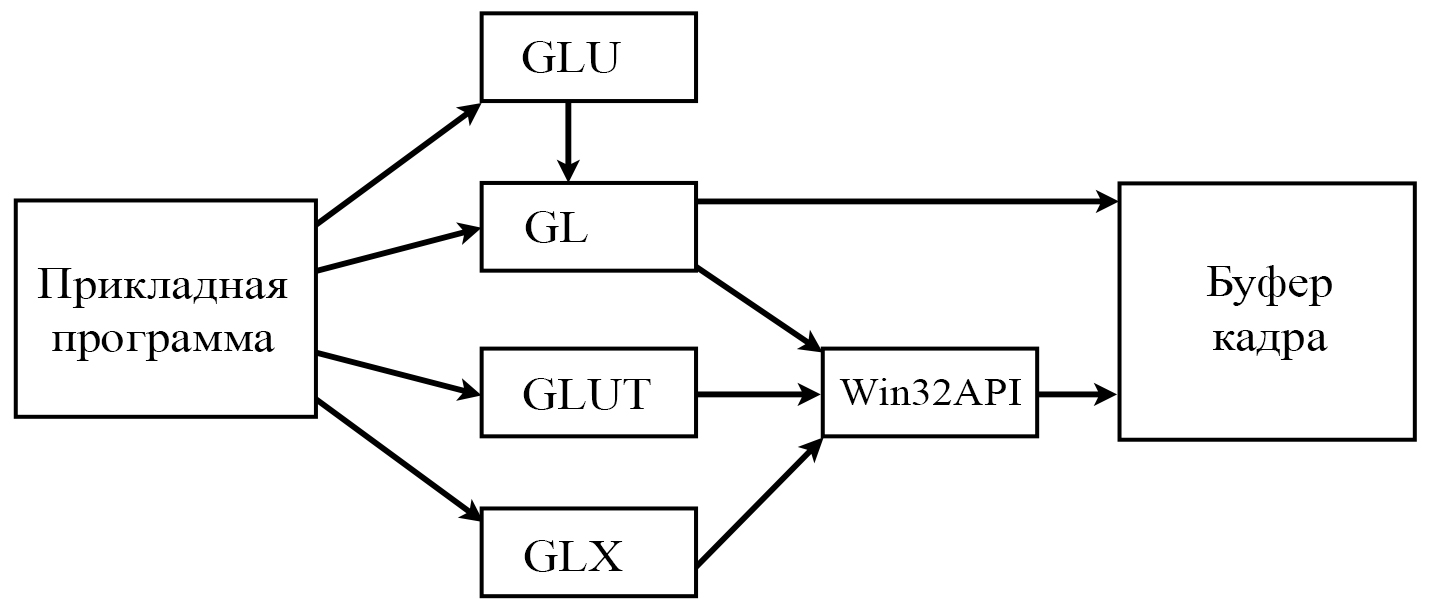
\includegraphics[width=1\linewidth]{diagram6.jpg}}
	\caption{Организация библиотеки OpenGL}
	\label{diagram6:image}
\end{figure}

Функции, специфичные для конкретной оконной подсистемы, обычно входят в ее прикладной программный интерфейс. Так, функции, поддерживающие выполнение OpenGL, есть в составе Win32 API и X Window. На рисунке схематически представлена организация системы библиотек в версии, работающей под управлением системы Windows. Аналогичная организация используется и в других версиях OpenGL.

\subsubsection{Архитектура OpenGL}

Функции OpenGL реализованы по принципу клиент-сервер. Приложение выступает в роли клиента – оно посылает команды, а сервер OpenGL интерпретирует и выполняет их. Сам сервер может находиться как на том же компьютере, на котором находится клиент (например, в виде динамически загружаемой библиотеки – DLL), так и на другом (при этом может быть использован специальный протокол передачи данных между машинами).

GL обрабатывает и рисует в буфере кадра графические примитивы с учетом некоторого числа выбранных режимов. Каждый примитив – это точка, отрезок, многоугольник и т.д. Каждый режим может быть изменен независимо от других. Определение примитивов, выбор режимов и другие операции описываются с помощью команд в форме вызовов функций прикладной библиотеки.

Примитивы определяются набором из одной или более вершин (vertex). Вершина определяет точку, конец отрезка или угол многоугольника. С каждой вершиной ассоциируются некоторые данные (координаты, цвет, нормаль, текстурные координаты и т.д.), называемые атрибутами. В подавляющем большинстве случаев каждая вершина обрабатывается независимо от других.

С точки зрения архитектуры графическая система OpenGL является конвейером, состоящим из нескольких последовательных этапов обработки графических данных.

Команды OpenGL всегда обрабатываются в том порядке, в котором они поступают, хотя могут происходить задержки перед тем, как проявится эффект от их выполнения. В большинстве случаев OpenGL предоставляет непосредственный интерфейс, т.е. определение объекта вызывает его визуализацию в буфере кадра.

С точки зрения разработчиков, OpenGL – это набор команд, которые управляют использованием графической аппаратуры. Если аппаратура состоит только из адресуемого буфера кадра, тогда OpenGL должен быть реализован полностью с использованием ресурсов центрального процессора. Обычно графическая аппаратура предоставляет различные уровни ускорения: от аппаратной реализации вывода линий и многоугольников до нестандартных и непривычных графических процессоров с поддержкой множеств операций над геометрическими данными.

\begin{figure}[H]
	\center{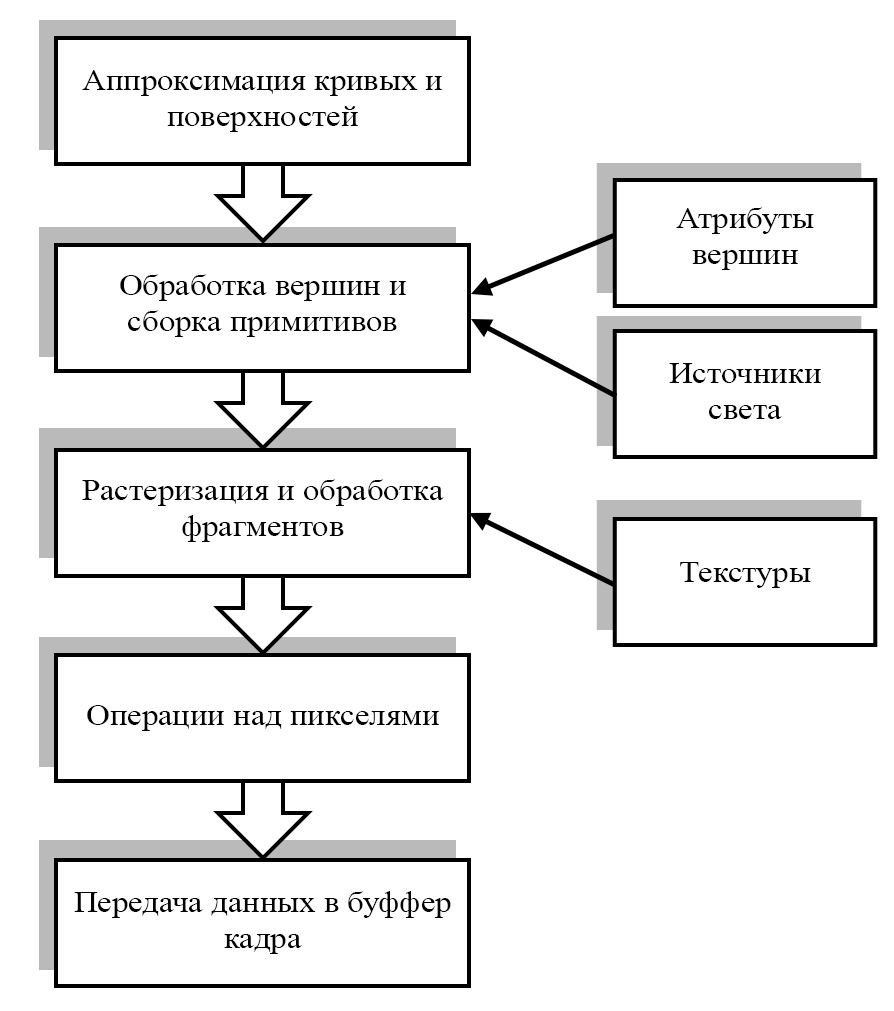
\includegraphics[width=0.7\linewidth]{diagram7.jpg}}
	\caption{Функционирование конвейера OpenGL}
	\label{diagram7:image}
\end{figure}

OpenGL является соединяющим звеном между аппаратурой и пользовательским уровнем, что позволяет предоставлять единый интерфейс на разных платформах, используя возможности аппаратной поддержки.

Кроме того, OpenGL можно рассматривать как конечный автомат, состояние которого определяется множеством значений специальных переменных и значениями текущей нормали, цвета, координат текстуры и других атрибутов и признаков. Вся эта информация будет использована при поступлении в графическую систему координат вершины для построения фигуры, в которую она входит. Смена состояний происходит с помощью команд, которые оформляются как вызовы функций.

\subsubsection{Работа с OpenTK}

OpenTK (Open набор средств) — это расширенная низкоуровневая библиотека C\#, которая упрощает работу с OpenGL, OpenCL и OpenAL. OpenTK можно использовать для игр, научных приложений или других проектов, требующих трехмерной графики, аудио или вычислительной функциональности.

Использование OpenTK предоставляет следующие возможности:
\begin{itemize}
	\item Быстрая разработка — OpenTK предоставляет надежные типы данных и встроенную документацию для улучшения рабочего процесса программирования и перехвата ошибок проще и быстрее;
	\item Простая интеграция — OpenTK была разработана для легкой интеграции с приложениями .NET;
	\item Разрешительная лицензия — OpenTK распространяется в соответствии с лицензиями MIT/X11 и полностью бесплатно;
	\item Расширенные привязки type-Сейф — OpenTK поддерживает последние версии OpenGL, OpenGL|ES, OpenAL и OpenCL с автоматической загрузкой расширений, проверка проверка и встроенной документацией;
	\item Гибкие параметры графического интерфейса — OpenTK предоставляет собственное, высокопроизводительные окно игры и приложения;
	\item Полностью управляемый, CLS-совместимый код . OpenTK поддерживает 32-разрядные и 64-разрядные версии macOS без неуправляемых библиотек;
	\item Трехмерные математические набор средств поставки Quaternion Vector Matrix OpenTK и Bezier структуры с помощью 3D-математических набор средств.
\end{itemize}

\subsection{Математика освещения в трёхмерной графике}

Для того, чтобы воссоздать искусственное освещение внутри моделируемого виртуального пространства, нам необходимо смоделировать поведение света при взаимодействии с различными поверхностями. Интересно, что эту задачу начал решать ещё в далеком в 18-м веке человек по имени Иоганн Генрих Ламберт.

В 1760 году швейцарский учёный выпустил книгу под названием Photometria. В ней он изложил фундаментальные правила поведения света; самым примечательным из них стало следующее — поверхность испускает свет (отражением или как источник освещения) таким образом, что яркость испускаемого света меняется в зависимости от косинуса угла между поверхностью нормали и наблюдателем.

\begin{figure}[H]
	\center{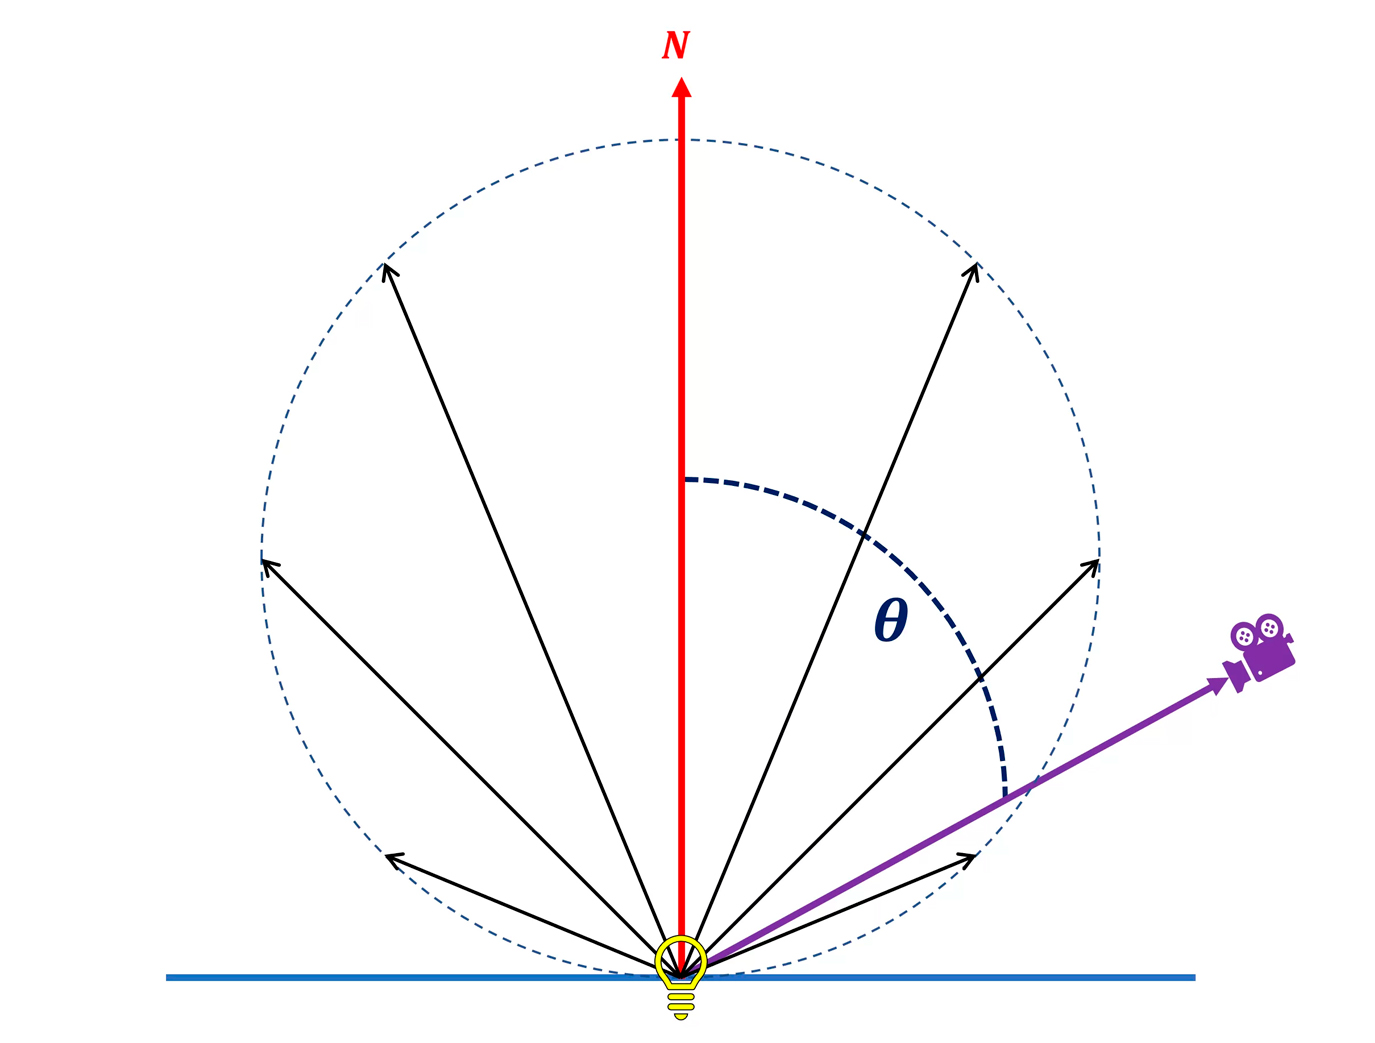
\includegraphics[width=0.8\linewidth]{diagram9.jpg}}
	\caption{Зависимость яркости отражаемого света поверхности от косинуса угла между нормалью и наблюдателем}
	\label{diagram9:image}
\end{figure}

\subsubsection{Рассеянный свет}

Это простое правило заложило основание определению рассеянного (diffuse light) освещения. Это математическая модель, используемая для вычисления цвета поверхности в зависимости от её физических свойств (например, её цвета и степени отражения света) и расположения источника освещения.

При 3D-визуализации для этого требуется некоторое множество параметров, что можно представить в виде такой схемы на рисунке ~\ref{diagram10:image}.

\begin{figure}[H]
	\center{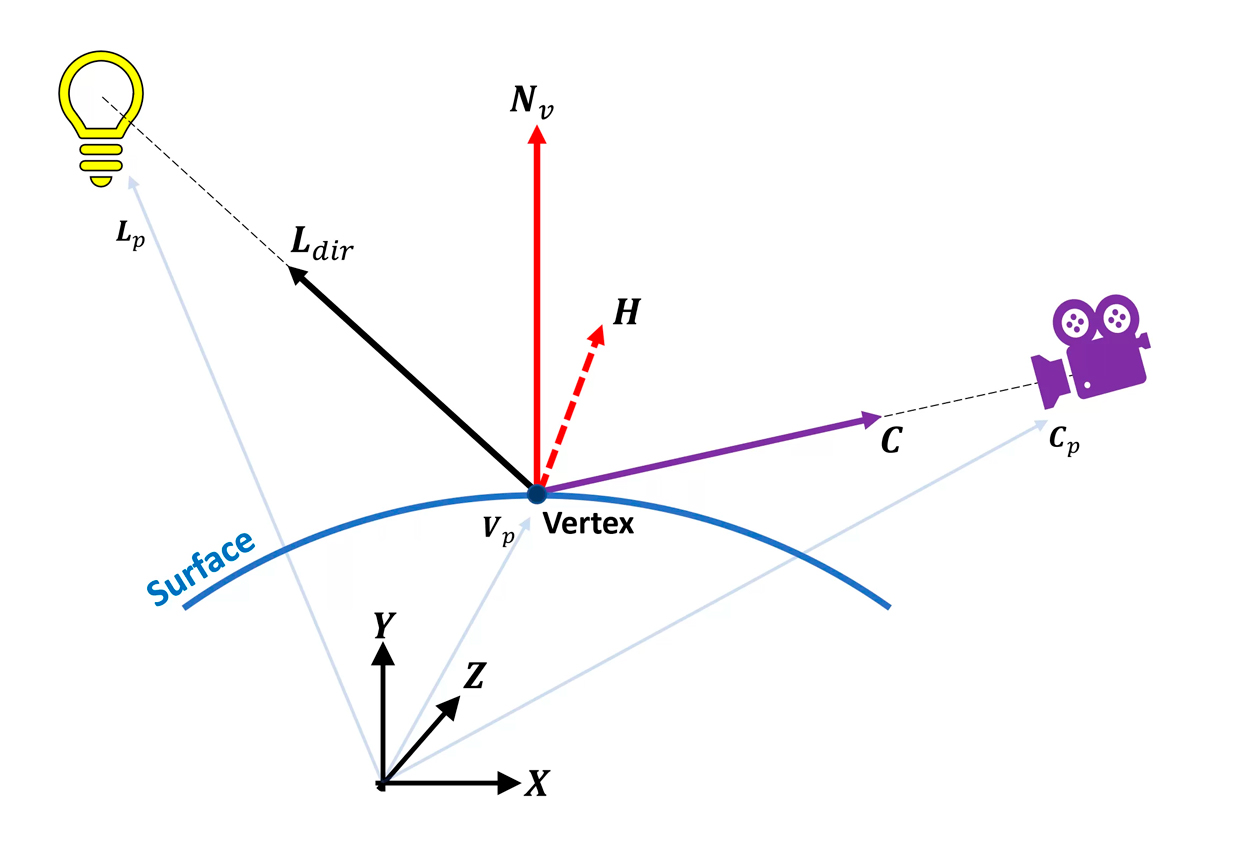
\includegraphics[width=0.8\linewidth]{diagram10.jpg}}
	\caption{Схема используемых параметров при 3D-рендеринге освещения}
	\label{diagram10:image}
\end{figure}

На изображении показано много указателей, это векторы, и для вычисления цвета отражения требуются следующие векторы:
\begin{itemize}
	\item 3 вектора для позиции вершины, источника освещения и камеры, смотрящей на сцену
	\item 2 вектора для направлений источника освещения и камеры с точки зрения вершины
	\item 1 вектор нормали (изображён красным)
	\item 1 полувектор (он всегда посередине между векторами направлений освещения и камеры)
\end{itemize}

Они вычисляются на этапе обработки вершин процесса рендеринга, а объединяющее их всех уравнение (называемое ламбертовой моделью) имеет вид:

\begin{figure}[H]
	\center{\hspace{10mm}{
\includegraphics[width=0.55\linewidth]{formula7.jpg}}}
\end{figure}

То есть, цвет вершины при рассеянном освещении вычисляется перемножением цвета поверхности, цвета источника освещения и скалярного произведения векторов нормали вершины и направления света с коэффициентами затухания и прожекторного освещения. Эта операция выполняется для каждого источника освещения в сцене, отсюда и символ суммы в начале уравнения.

Всё это нужно для вычисления значения рассеянного освещения и все эти операции требуется выполнять для каждого источника освещения в виртуальной сцене, или, по крайней мере, для каждого источника, который существует на сцене и обрабатывается программой. Многие из этих уравнений выполняются графическими API, но их можно выполнять и вручную, если необходимо реализовывать более сложные операции над изображением.

\subsubsection{Общий свет}

Но помимо рассеянного света существует бесконечное множество других видов освещений, и каждая поверхность отражает свет, поэтому все они влияют на общее освещение сцены. Даже ночью присутствует фоновое освещение, будь то звёзды и планеты или свет, рассеивающийся в атмосфере.

Для моделирования реалистичного света, вычисляется ещё одно значение освещения: ambient lighting (освещение окружающей среды), или же общий свет.

\begin{figure}[H]
	\center{\hspace{10mm}{
\includegraphics[width=0.55\linewidth]{formula8.jpg}}}
\end{figure}

Это уравнение проще, чем для рассеянного освещения, потому что не требуются направления. Здесь выполняется простое перемножение различных коэффициентов:

\begin{itemize}
	\item C$_S$$_A$ — цвет подсветки поверхности
	\item C$_G$$_A$ — цвет подсветки глобальной 3D-сцены
	\item C$_L$$_A$ — цвет подсветки всех источников освещения в сцене
\end{itemize}

\subsubsection{Отраженный свет}

Определив фоновое освещение и введя в расчет рассеянный свет источников освещения от различных поверхностей 3D-мира, виртуальное освещение начинает выглядеть намного более реалистично. Но модель Ламберта работает только для материалов, которые отражают освещение от своей поверхности во всех направлениях. Объекты, изготовленные из стекла или металла, создают другой тип отражения, называемый зеркальным (specular). И для него тоже необходимо определить уравнение.

\begin{figure}[H]
	\center{\hspace{10mm}{
\includegraphics[width=0.55\linewidth]{formula9.jpg}}}
\end{figure}

Отдельные части этой формулы уже были определены раннее: имеется два значения зеркального цвета (одно для поверхности — C$_{S}$, другое для света — C$_{LS}$), а также привычные коэффициенты затухания и прожекторности.

Так как зеркальное отражение очень сфокусировано и направлено, для определения яркости зеркального освещения используются два вектора: нормаль вершины и полувектор. Коэффициент $p$ называется мощностью зеркального отражения, это число, определяющее яркость отражения в зависимости от свойств материала поверхности. При увеличении $p$ зеркальный эффект становится ярче, но более сфокусированным и меньшим по размерам.

\subsubsection{Испускаемый свет}

Последний учитываемый элемент — самый простой, потому что математически представляется лишь одним числом. Оно называется испускаемым (emissive) освещением, и применяется к объектам, являющимся непосредственным источником освещения, то есть к пламени, фонарику или Солнцу.

Это означает, что на данный момент определены одно число и три набора уравнений для вычисления цвета вершины поверхности, учёта фонового освещения (окружающей среды), а также взаимодействия между различными источниками освещения и свойствами материала поверхности (diffuse и specular). В программной среде можно использовать либо только один или же скомбинировать все четыре источника света, просто сложив их вместе:
\begin{figure}[H]
	\center{\hspace{10mm}{
\includegraphics[width=0.35\linewidth]{formula10.jpg}}}
\end{figure}

Визуально сочетание различных видов света выглядит так:

\begin{figure}[H]
	\center{\hspace{10mm}{
\includegraphics[width=1\linewidth]{diagram11.jpg}}}
	\caption{Визуальное представление результата наложения нескольких типов освещений на одном объекте}
	\label{diagram11:image}
\end{figure}

\subsection{Аффинные преобразования трёхмерного пространства}

При работе с трёхмерными объектами, часто требуется совершать по отношению к ним различные преобразования: двигать, поворачивать, сжимать, растягивать, скашивать и т.д. При этом в большинстве случаев требуется, чтобы после применения этих преобразований сохранялись определенные свойства.

Преобразование плоскости называется аффинным (от англ. affinity – родство), если
\begin{itemize}
	\item оно взаимно однозначно;
	\item образом любой прямой является прямая.
\end{itemize}

Преобразование называется взаимно однозначным, если
\begin{itemize}
	\item разные точки переходят в разные;
	\item в каждую точку переходит какая-то точка.
\end{itemize}

Свойства аффинного преобразования в трехмерном пространстве:
\begin{itemize}
	\item отображает n-мерный объект в n-мерный: точку в точку, линию в линию, поверхность в поверхность;
	\item сохраняет параллельность линий и плоскостей;
	\item сохраняет пропорции параллельных объектов – длин отрезков на параллельных прямых и площадей на параллельных плоскостях.
\end{itemize}

Любое аффинное преобразование задается матрицей 3x3 с ненулевым определителем и вектором переноса:
\begin{figure}[H]
	\center{
\includegraphics[width=0.6\linewidth]{formula1.jpg}}
\end{figure}

\subsubsection{Параллельный перенос}
\begin{figure}[H]
	\center{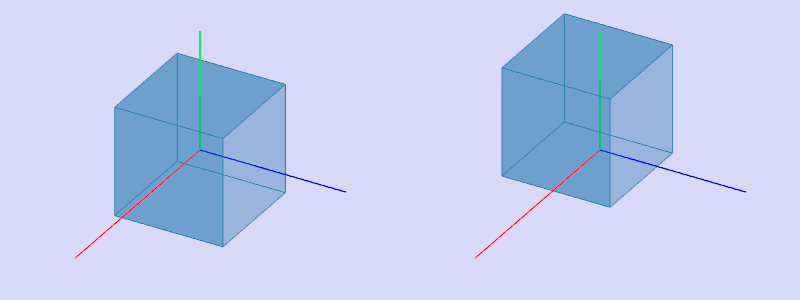
\includegraphics[width=1\linewidth]{prim1.jpg}}
	\caption{Преобразование вида параллельный перенос}
	\label{prim1:image}
\end{figure}

Матрица этого преобразования выглядит следующим образом:

\begin{figure}[H]
	\hspace{10mm}{
\includegraphics[width=0.25\linewidth]{formula2.jpg}}
\end{figure}

В данном случае матрица R = E, единичной матрице.

\subsubsection{Поворот вокруг оси}
\begin{figure}[H]
	\center{
\includegraphics[width=1\linewidth]{prim2.jpg}}
	\caption{Преобразование вида поворот вокруг оси}
	\label{prim2:image}
\end{figure}

Заметим, что при повороте вокруг оси y ординаты точек (у-координаты) не меняются. Также стоит отметить, что координаты x и z точки преобразуются независимо от y-координаты. Это означает, что любая точка p(x, y, z) перейдет в точку p’(x’(x, z), y, z’(x, y)). Теперь осталось понять, как преобразуются координаты x и z: в плоскости Oxz это будет поворот вокруг начала координат по часовой стрелке (т.к. x z y - левая тройка), т.е. в отрицательном направлении. Матрица такого преобразования известна:
\begin{figure}[H]
	\hspace{10mm}{
\includegraphics[width=0.43\linewidth]{formula3.jpg}}
\end{figure}

\vspace*{5mm}Матрица преобразования Ry(φy):

\begin{figure}[H]
	\hspace{10mm}{
\includegraphics[width=0.43\linewidth]{formula4.jpg}}
\end{figure}

\subsubsection{Масштабирование}
\begin{figure}[H]
	\center{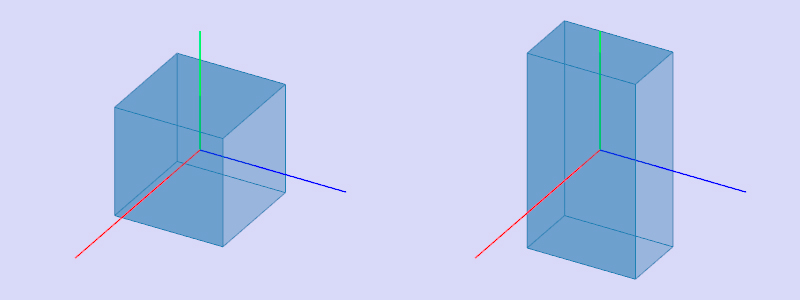
\includegraphics[width=1\linewidth]{prim3.jpg}}
	\caption{Преобразование вида масштабирование}
	\label{prim3:image}
\end{figure}

Коэффициенты сжатия/растяжения, по аналогии с двухмерным пространством, определяются диагональными членами матрицы R:
\begin{figure}[H]
	\hspace{10mm}{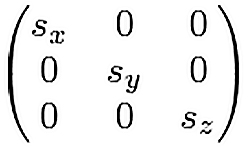
\includegraphics[width=0.2\linewidth]{formula5.jpg}}
\end{figure}

\vspace*{5mm}Результат:

\begin{figure}[H]
	\hspace{10mm}{
\includegraphics[width=0.2\linewidth]{formula6.jpg}}
\end{figure}

Комбинация коэффициентов $s_x$ = -1, $s_y$ = 1, $s_z$ = 1 будет задавать отражение от плоскости Oyz (x = 0). При $s_x$ = $s_y$ = $s_z$ = -1 получим центральную симметрию относительно начала координат.
\section{Техническое задание}
\subsection{Основание для разработки}

Основанием для разработки является задание на производственную преддипломную практическую работу в компании "<ООО МЦОБ. Онлайн Сервисы">.

\subsection{Цель и назначение разработки}

Основной задачей производственной преддипломной практической работы является разработка программной системы для визуализации трёхмерных данных, использующая библиотеку OpenGL.

Используя библиотеку OpenGL последней версии, планируется разработать приложение на языке C\#, способное импортировать массив трёхмерных данных и визуализировать их в виде трёхмерных моделей.

Задачами данной разработки являются:
\begin{itemize}
\item создание программы, реализующей графику, на основе спецификации OpenGL;
\item реализация программы парсера, способного преобразовывать и загружать в программу трёхмерные данные;
\item разработка интерфейса для взаимодействия с программой;
\item реализация функции хранения и загрузки трёхмерных данных внутри программы.
\end{itemize}

\subsection{Требования к программной системе}

\subsubsection{Требования к данным программно-информационной системы}

Входными данными для программной системы являются файлы с расширением *.obj, внутри которых содержатся информация в виде массивов трёхмерных данных; файлы текстур - изображения с расширением *.png и *.jpg; данные ввода с клавиатуры и мыши, которые служат для управления перемещением и вращением камеры.

Выходными данными для программной системы является выводимое на экран изображение двумерной проекции трёхмерных объектов на виртуальной сцене.

На рисунке ~\ref{diagram1:image} представлена диаграмма описания потоков данных в программе.

\begin{figure}[ht]
	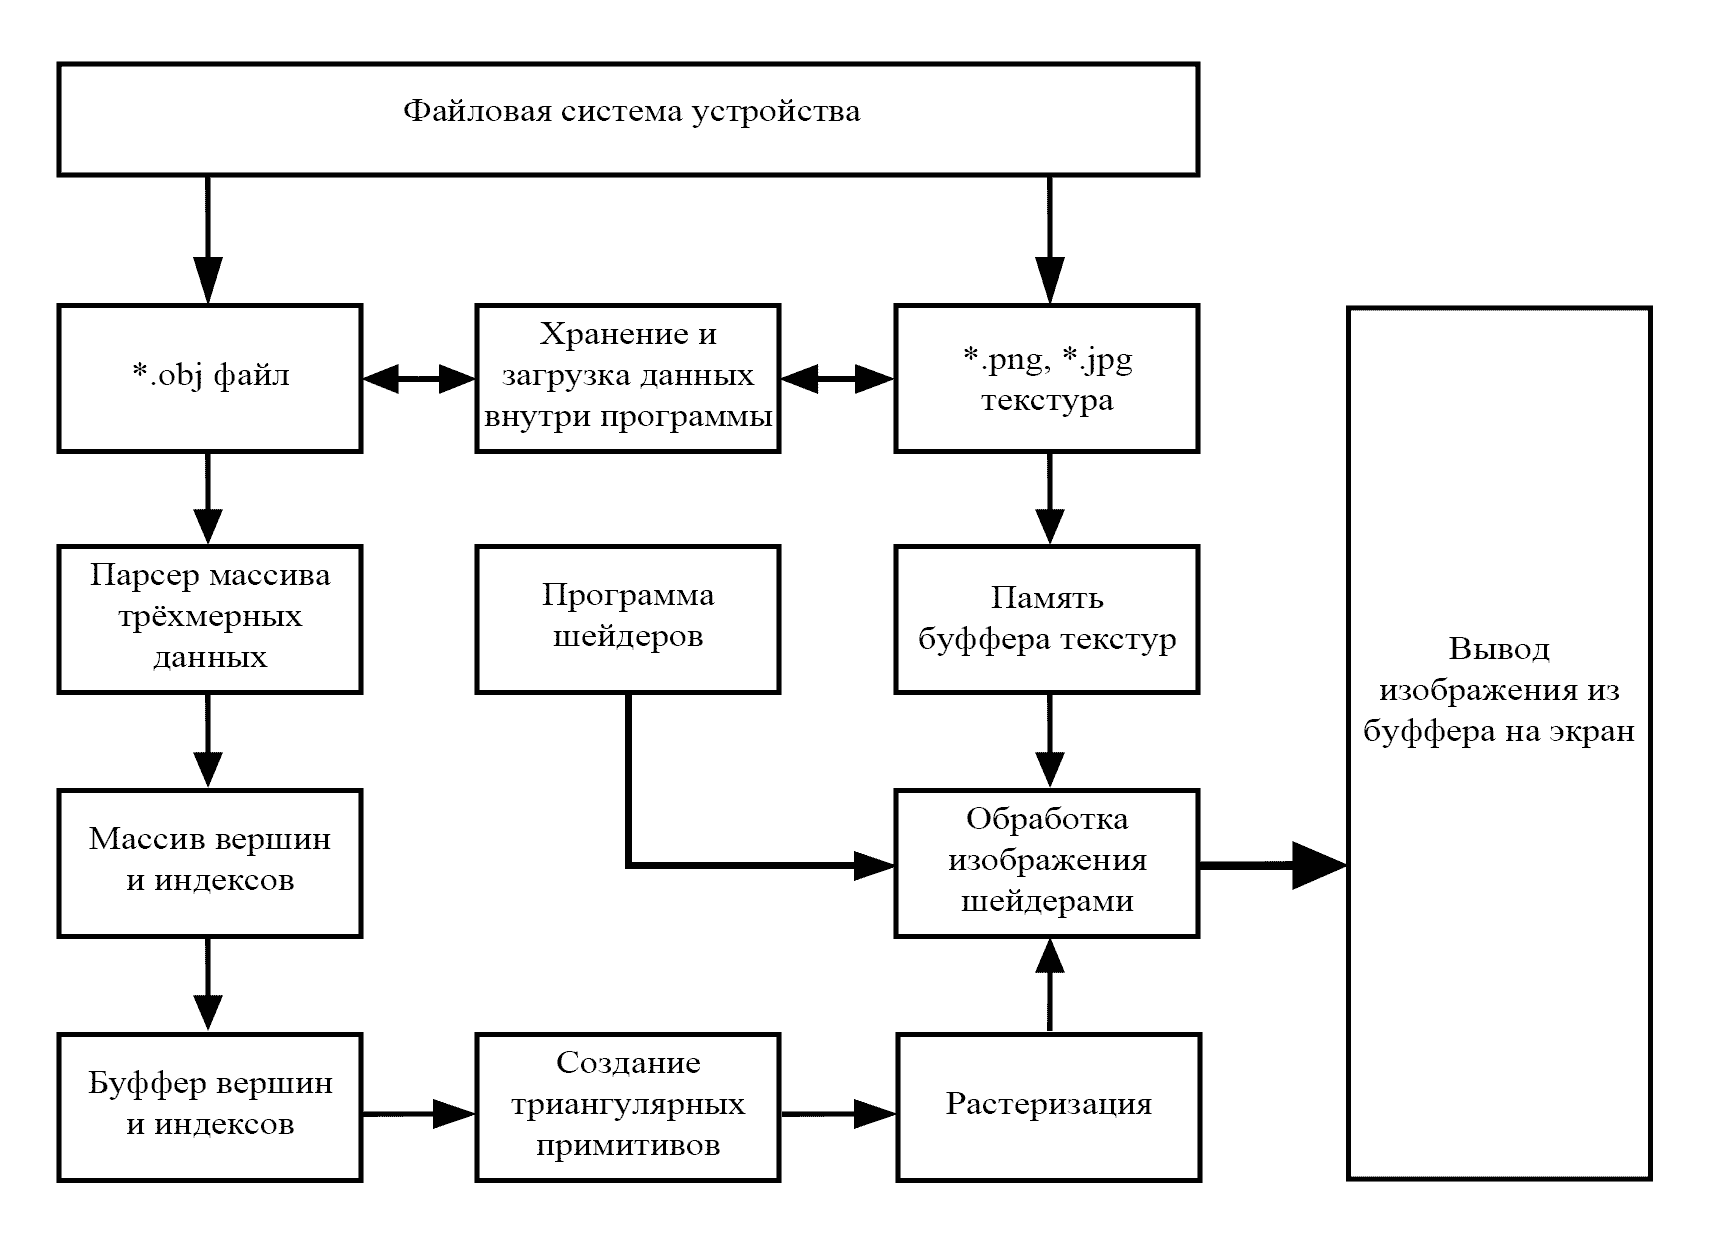
\includegraphics[width=1\linewidth]{diagram1}
	\caption{Диаграмма потоков данных в программе}
	\label{diagram1:image}
\end{figure}

\subsubsection{Функциональные требования к программной системе}

Программа должна реализовывать следующие функции:
\begin{itemize}
    \item позволять пользователю импортировать любые массивы трёхмерных данных (включая текстуры для трёхмерных моделей);
    \item выполнять отрисовку трёхмерной сцены в реальном времени (каждый кадр);
    \item пользволять пользователю свободно управлять перспективой виртуальной камеры;
    \item предоставлять возможность преобразовывать массив трёхмерных данных (производить аффинные преобразования) в рамках: сдвига, вращения и растяжения (сжатия);
    \item импортировать, хранить и загружать массив трёхмерных данных внутри самой программы.
\end{itemize}



Виды преобразований массива трёхмерных данных, предоставляемых программой, представлены на рисунке ~\ref{affin:image}.

\begin{figure}[ht]

\includegraphics[width=1\linewidth]{affin}
\caption{Виды преобразований массива трёхмерных данных}
\label{affin:image}
\end{figure}
%\vspace{-\figureaboveskip} % двойной отступ не нужен (можно использовать, если раздел заканчивается картинкой)

\subsubsection{Требования к графическому интерфейсу программы}

Программное обеспечение должно иметь минимальный, но содержательный и интуитивный интерфейс. Большую часть основного окна приложения должно занимать само окно вывода растрового изображения проекции виртуальной сцены и всех трёхмерных данных на ней. Сбоку на основном окне приложения должно находиться специально выведенное отдельное окно «инспектора», с помощью которого пользователь сможет управлять загрузкой и сохранением массивов трёхмерных данных, а также взаимодействовать с уже существующими данными на виртуальной сцене.

Макет пользовательского интерфейса, составленный по данным требованиям представлен на рисунке ~\ref{maket1:image}

\begin{figure}[ht]
	
\includegraphics[width=1\linewidth]{maket1}
	\caption{Макет пользовательского интерфейса}
	\label{maket1:image}
\end{figure}

\subsection{Моделирование вариантов использования}

Для разрабатываемого программного обеспечения была реализована модель, которая демонстрирует наглядное представление вариантов использования программы.

На основании анализа предметной области в программе должны быть реализованы следующие прецеденты:
\begin{enumerate}
\item Импортирование массивов трёхмерных данных из файловой системы пользователя.
\item Просмотр визуализированного массива трёхмерных данных в виде отрисованных объектов на экране.
\item Осуществление трансформаций над массивом трёхмерных данных.
\item Хранение и загрузка массивов трёхмерных данных.
\end{enumerate}

На рисунке ~\ref{diagram2:image} представлена диаграмма вариантов использования

\begin{figure}[H]
	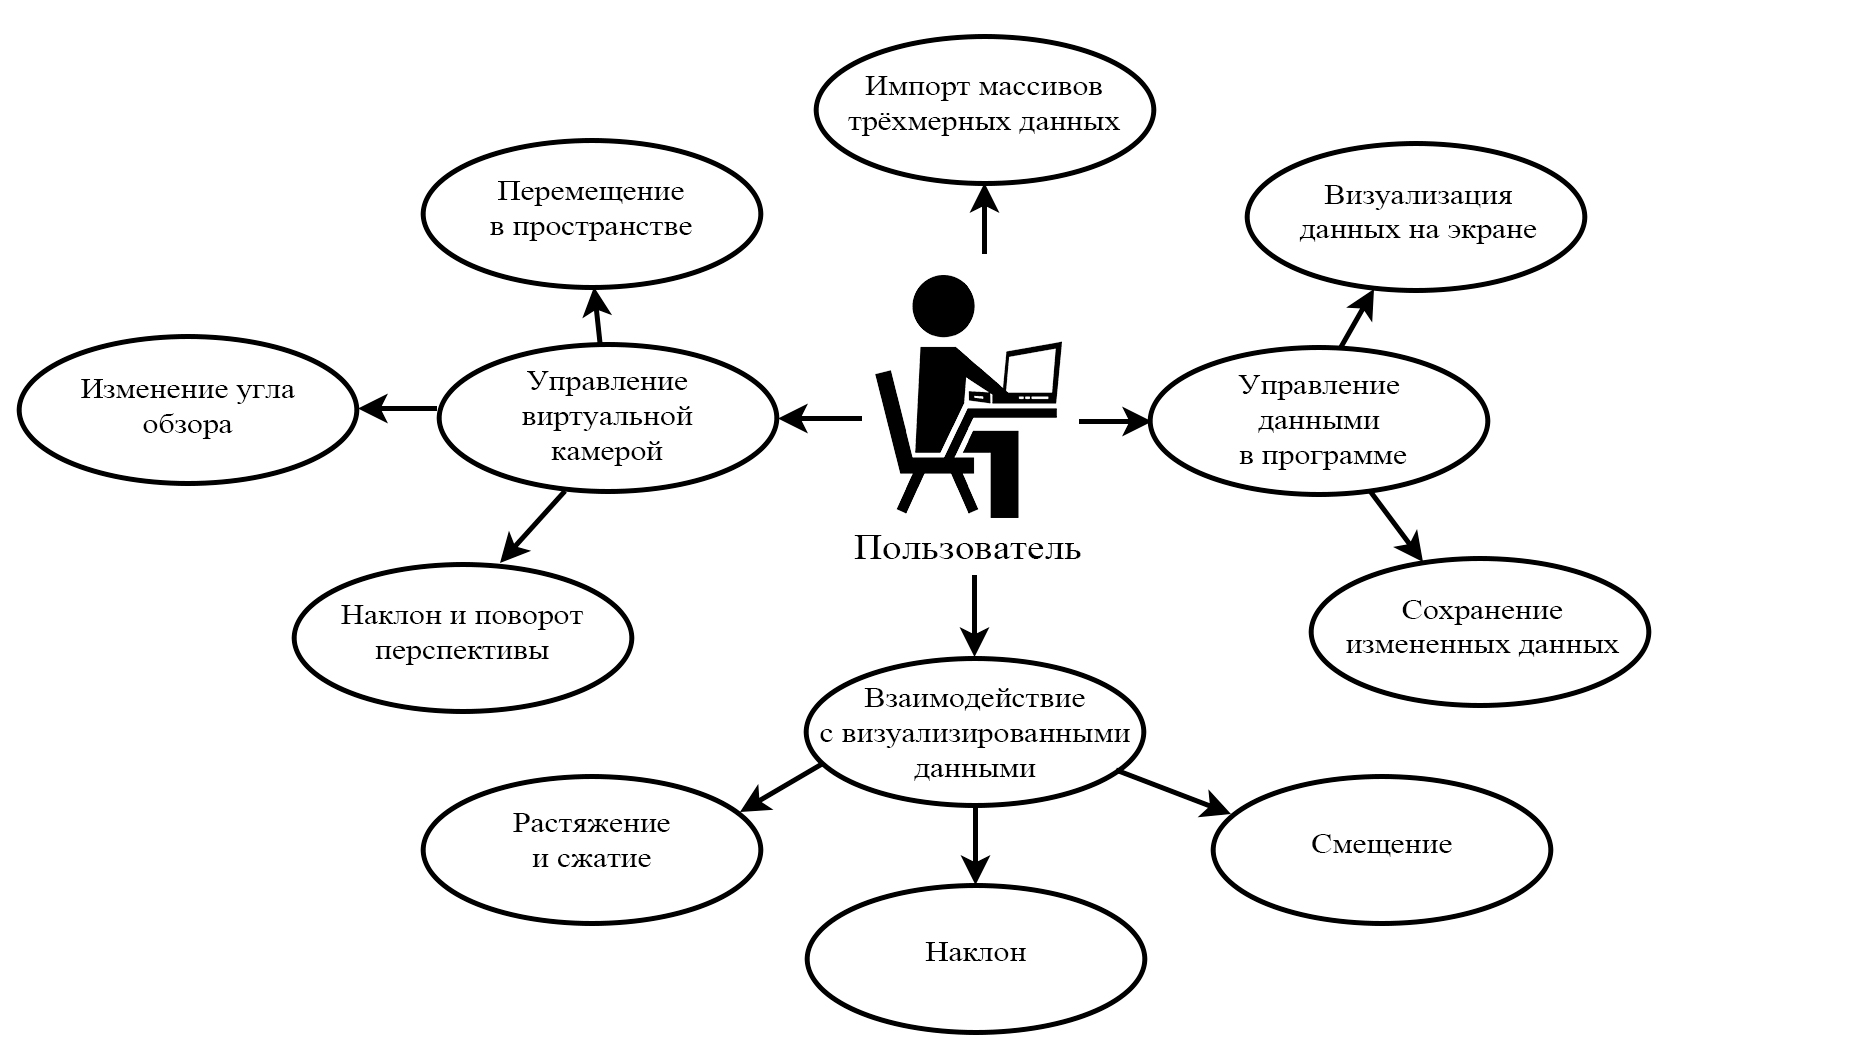
\includegraphics[width=1.1\linewidth]{diagram2}
	\caption{Диаграмма вариантов использования}
	\label{diagram2:image}
\end{figure}

\subsection{Нефункциональные требования к программной системе}

Требования к аппаратной совместимости:
\begin{itemize}
	\item видеоадаптер с поддержкой OpenGL версии не ниже 4.6;
	\item минимальное разрешение экрана - 800х600 пикселей.
\end{itemize}

Требования к программной совместимости:
\begin{itemize}
	\item операционная система x86 Windows 7 и выше;
	\item система, с установленными компонентами Microsoft Visual C++ версии 2015 года и выше.
\end{itemize}

\subsection{Требования к оформлению документации}

Разработка программной документации и программного изделия должна производиться согласно ГОСТ 19.102-77 и ГОСТ 34.601-90. Единая система программной документации.


\section{Технический проект}
\subsection{Общая характеристика организации решения задачи}

Поставлена цель разработать программу, работающую на спецификации OpenGL, способную загрузить массив трёхмерных данных и графически осуществить их визуализацию на экране для пользователя.

Трёхмерный графический движок на высоком уровне является программным движком, основной задачей которого является визуализация трёхмерной компьютерной графики, представляет из себя структуру основных классов - примитивов, являющихся основой трёхмерной графики: массив координат точек, массив нумерации граней, матрица проекциий, объект виртуальной камеры, набор текстур и программ шейдеров, которые все вместе осуществляют отрисовку объекта на трёхмерной сцене.

На более низком уровне трёхмерный движок представляет из себя набор комманд и программ для работы с видеоадаптерами и буфферами памяти системы. Из данного набора команд и программ была создана основа разрабатываемой программы, работающей под спецификацией OpenGL.

В движке используется разработанная программа парсера. Парсер считывает структуру файлов трёхмерных объектов. Массив трёхмерных данных считывается последовательно и обрабатываются синтаксическим анализатором. На основе данных считанных объектов формируются массивы координат вершин, индексов и координат текстур.
\subsection{Обоснование выбора технологии проектирования}

Обоснованием выбора технологии проектирования послужило задание на разработку, целью которой являлось создание программы, работающей на спецификации OpenGL. Соответственно, была выбрана последняя выпущенная версия OpenGL 4.6. А выбором среды и языка проектирования интерфейса и создания программы являлось наличие необходимых функций для проектирования интерфейса и программы графического движка у языка C\# в среде Visual Studio.

\subsection{Описание используемых технологий и языков программирования}

В процессе разработки программного обеспечения было использовано программное средство IDE Visual Studio, а также использованы языки программирования C\# - при создании интерфейса программы, C - при работе со спецификацией OpenGL, графическая библиотека OpenGL и библиотека OpenTK для упрощения работы и адаптации OpenGL на платформы Mono и .NET на языке C\#.

\subsubsection{Язык программирования C\#}

\paragraph{Особенности языка C\#}

C\# - многоцелевой объектно-ориентированный язык программирования. Относится к семье с С-подобным синтаксисом, наиболее идентичен C++ и Java. Имеет более расширенный спект функций, чем у предшественника - C++, чем является намного проще в использовании, но также из-за своих удобств является более высокоуровневым, что делает его ориентированным в основном на разработку десктопных приложений.

Язык C\# является немного более высокоуровневым, чем C++, поэтому менее тесно взаимодействует с аппаратной частью вычислительных систем, что в какой-то степени ограничивает его функционал в случаях разработки низкоуровневых приложений, где работа с памятью системы и прямое взаимодействие с аппаратной частью необходимо.

\subsubsection{Спецификация OpenGL 4.6}

OpenGL ориентирован на две задачи:
\begin{itemize}
	\item Скрыть сложности адаптации различных 3D-ускорителей, предоставляя разработчику единый API;
	\item Скрыть различия в возможностях аппаратных платформ, требуя реализации недостающей функциональности с помощью программной эмуляции.
\end{itemize}

\paragraph{Особенности спецификации OpenGL}

\begin{itemize}
	\item Гибкость, открытый код и низкие требования к ресурсам устройства;
	\item возможности данной спецификации позволяют разработчику создавать полностью уникальные и подстроенные под особую специфику задач приложения;
	\item устройство данной графической библиотеки позволяет запускать и поддерживать приложения с максимально возможной производительностью;
	\item это низкоуровневая библиотека, которая позволяет напрямую работать с аппаратным железом - управлять памятью системы и буфером видеоадаптера;
	\item самодостаточность спецификации даёт возможность не использовать дополнительные плагины и библиотеки в реализации визуализации графики;
	\item полная мультиплатформенность - OpenGL работает на всех платформах, языках и устройствах;
	\item низкоуровневость библиотеки - для неопытного, или же начинающего разработчика это может стать главной проблемой в работе с OpenGL, потому как для создания программного обеспечения, использующего спецификацию OpenGL, необходимы глубокие знания об основах трёхмерной графики и линейной алгебры, а также иметь минимальное представление об обмене данными в видеоадаптерах на аппаратном уровне;
	\item данная технология в настоящее время считается уже устаревшей, и была заменена более современным API Vulcan;
	\item с выходом новых видеокарт, их спектр возможностей, как и реализуемых функций расширился, так что новые функции, такие как DLSS и RTX не вошли в стандарт спецификации OpenGL.
	
\end{itemize}

\subsection{Диаграмма классов и компонентов программы}

\subsubsection{Диаграмма классов}

Диаграмма классов описывает виды классов программы и различного рода связи, которые существуют между элементами. На диаграммах изображаются также атрибуты классов, их функции, принимаемые значения, а также ограничения описывающие взаимодействие между классами. Вид и представление диаграммы классов напрямую зависит от уровня абстракции: классы могут быть показаны в качестве сущностей предметной области или же как элементы частей программного обеспечения. В нашем случае, на рисунке \ref{diagram3:image} показана диаграмма классов, которые являются элементами программной среды. 

Атрибуты в диаграмме описывают свойства объектов класса. Элементы класса обладают своей индивидуальностью из-за различий в их параметрах, а также связях с другими объектами. 

В большинстве случаев, в данном программном обеспечении большинство классов существуют в единственном экземпляре, из-за их уникальной сущности. Как пример, можно привести класс, определяющий виртуальную камеру, которая должна существовать в единственном экземпляре, ведь на один экран должно выводиться одновременно лишь одно изображение.

Но несмотря на это, структура классов в данном программном обеспечении всё равно является объектно ориентированной, благодаря чему внутри неё был реализован механизм управления объектными моделями, текстурами и другими элементами, которые все связаны между собой наследуемостью классов, а также существует возможность дальнейшего развития и расширения общей системы классов, путём добавлением в неё новых элементов.

\begin{figure}[H]
\center{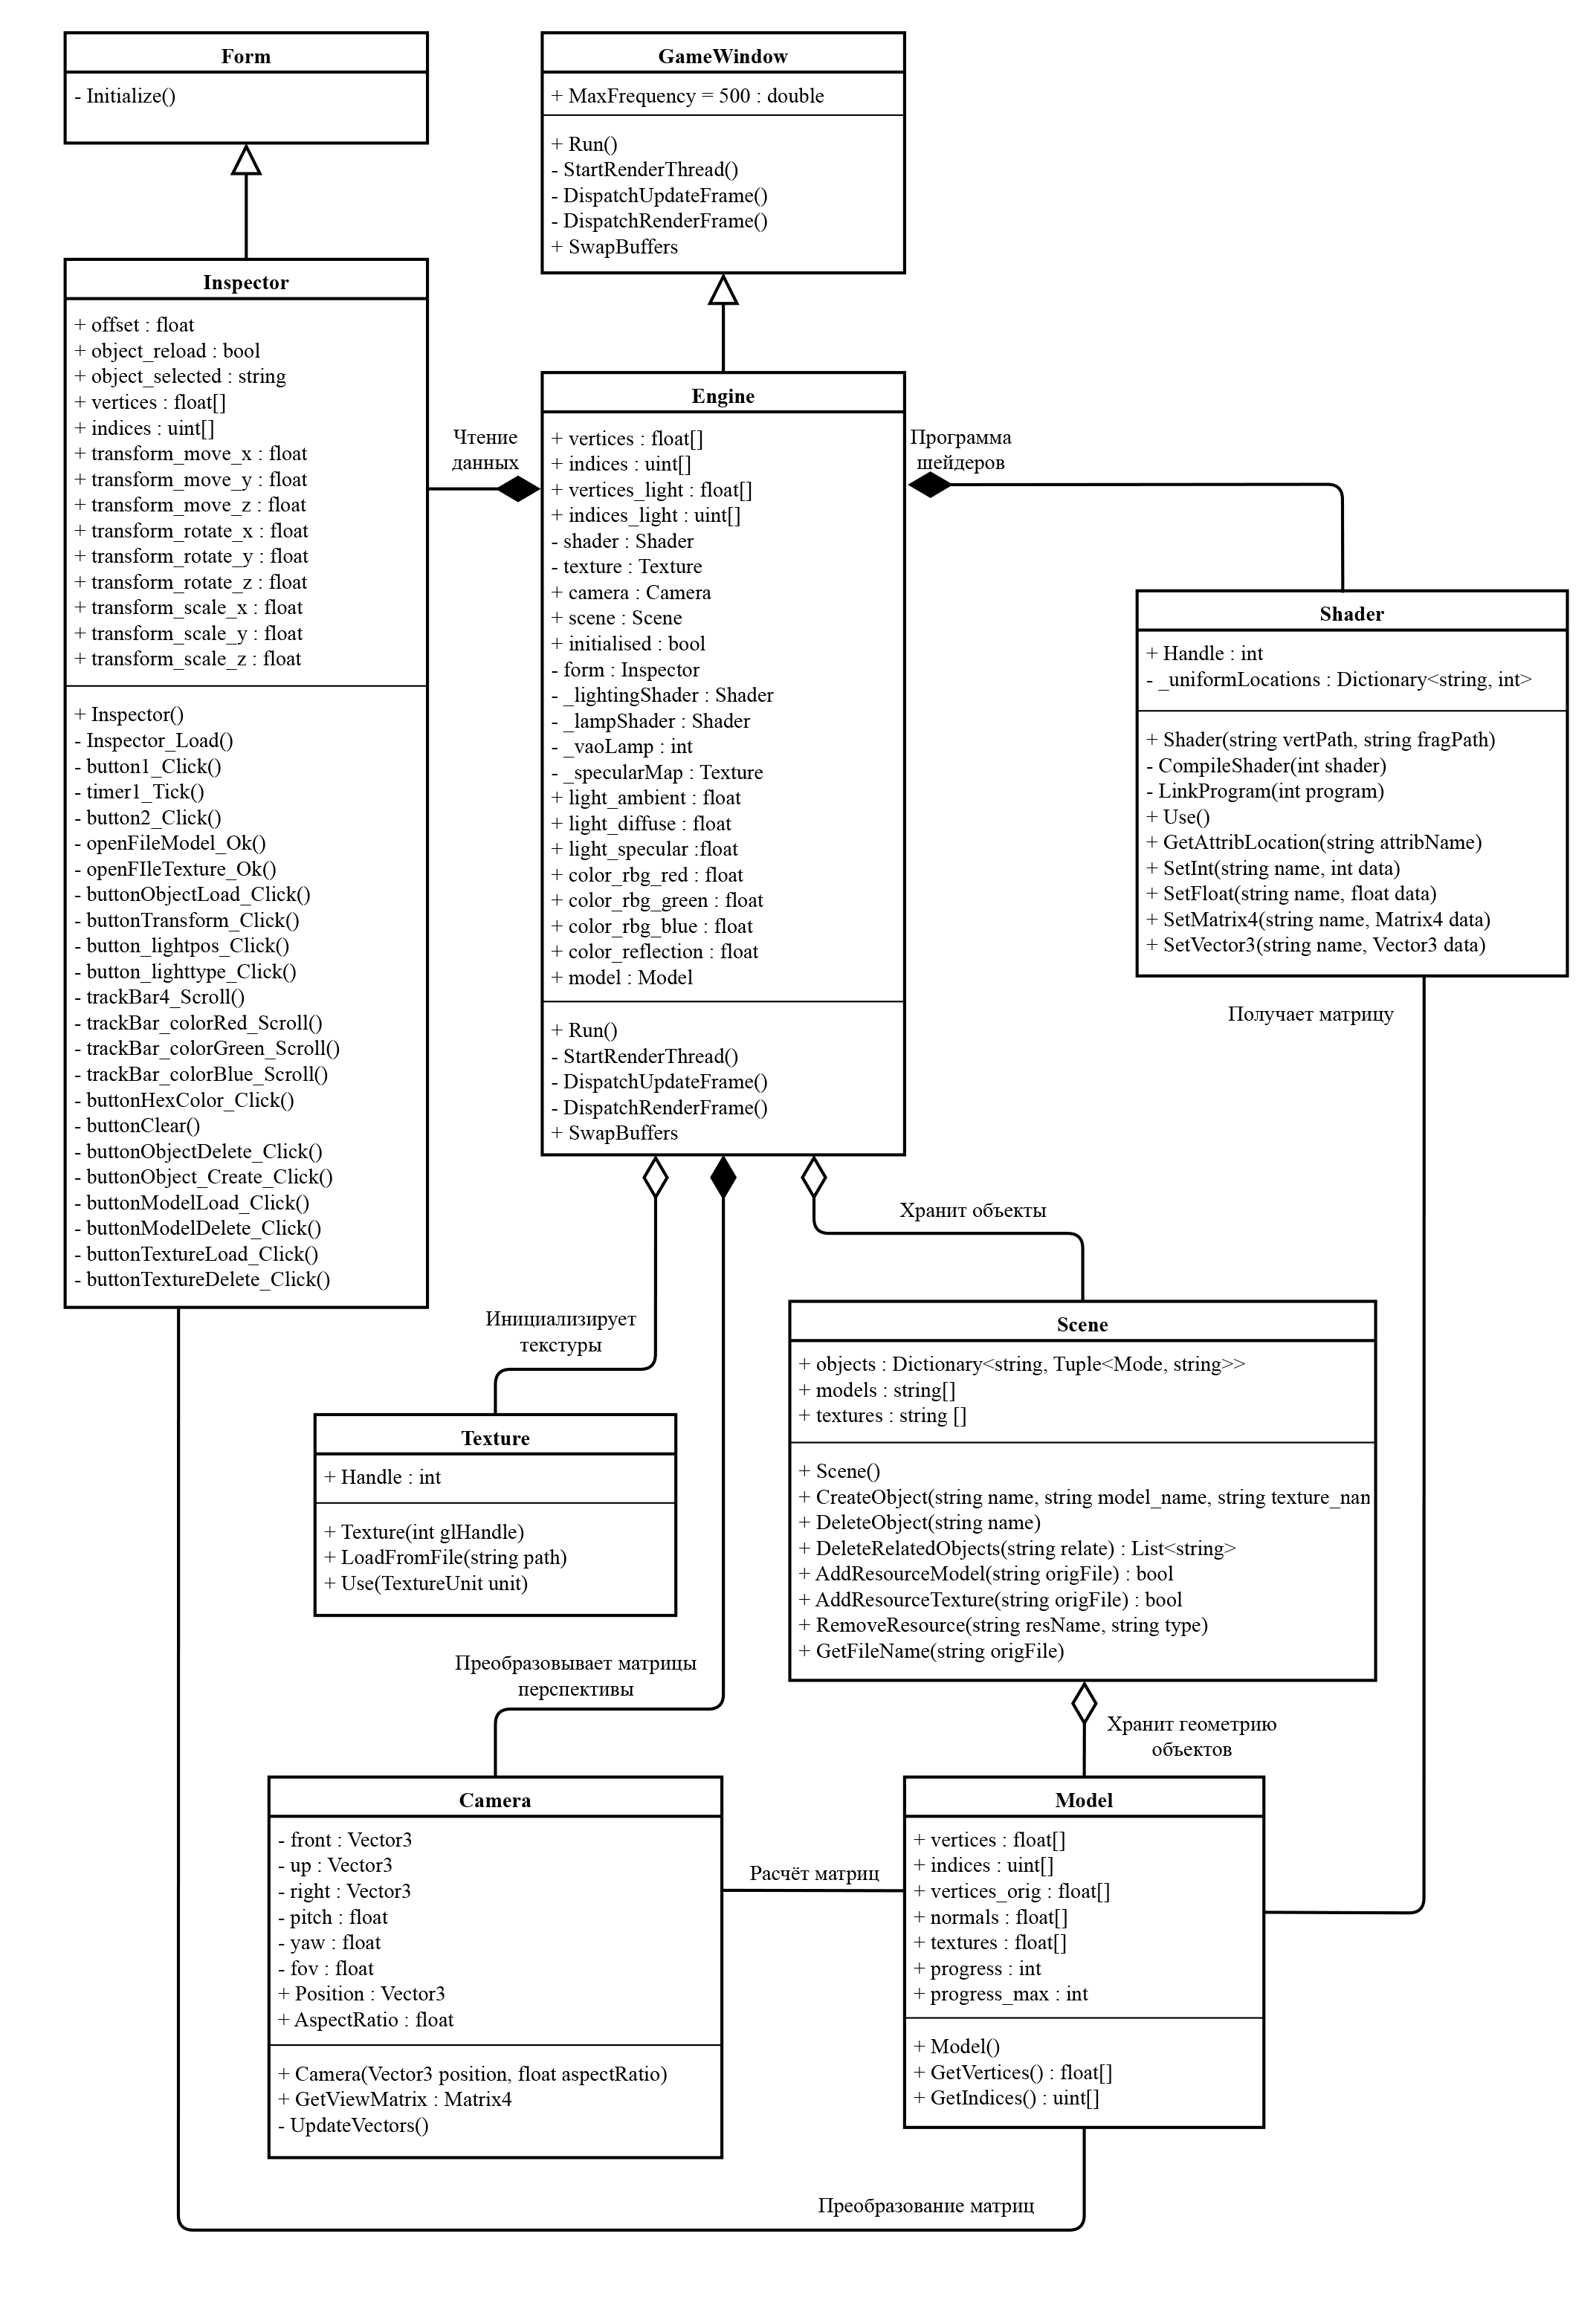
\includegraphics[width=1\linewidth]{diagram12.png}}
\caption{Диаграмма классов программы}
\label{diagram3:image}
\end{figure}

Все элементы программы имеют общий родительский элемент в виде главного класса - обработчика событий, который является главным элементом и центром всей программы.

\paragraph{Класс Model}

Является каркасом трёхмерной модели. Выполняет роль приёма, хранения и передачи массива трёхмерных данных для обработчика триангулярных примитивов. При создании выполняет чтение и преобразование в массивы вершин и индексов, загруженного файла с данными трёхмерного объекта.

\paragraph{Класс Texture}

При инициализации выделяет место в буффере памяти видеоадаптера для загруженной в программу текстуры, а также обрабатывает настройки параметров её отображения;

\paragraph{Класс Scene}

Выполняет роль хранилища моделей и изображений, а также выступает виртуальной сценой, на которой находятся все трёхмерные объекты и остальные элементы, учавствующие в визуализации. При инициализации выполняет загрузку данных массивов моделей и привязанных к ним файлов текстур, которые уже были раннее загружены в проект;

\paragraph{Класс Shader}

Программа настройки конечной визуализации, и при инициализации создаёт подпрограмму в общей графике, для преобразования растеризированного изображения внутри буффера памяти видеоадаптера, для отображения текстур и освещения;

\paragraph{Класс Camera}

Является матрицей преобразования, для корректного отображения перспективы виртуального трёхмерного вида сцены, и для того, чтобы конечный вид проекции сцены был перспективным, а не ортографическим;

\paragraph{Класс Model}

Представляет из себя основу проекта - графический движок, который инициализирует всю графику, принимает события ввода пользователя, отвечает за обновление кадров и управление всеми настройками, а также связывает все классы между собой;

\paragraph{Класс Inspector}

Часть пользовательского интерфейса, представляющего из себя окно взаимодействия между пользователем и программой. Служит для того, чтобы пользователь осуществлял загрузку собственных массивов трёхмерных данных моделей и текстур в проект, а также осуществлял указанные аффинные преобразования над загруженными моделями.

\paragraph{Класс GameWindow}

Также отдельно стоит указать класс GameWindow - это родительский класс для класса Engine. По своей сути он является измененным элементом класса Form от WindowsForms и не принимает прямого участия в работе проекта, но содержит формальные данные, необходимые для корректной инициализации главного окна проекта.

\subsubsection{Диаграмма компонентов}

Диаграмма компонентов - это структурная диаграмма языка унифицированного моделирования, она описывает особенности физического представления системы. Диаграмма компонентов позволяет определить архитектуру разрабатываемой системы, установив зависимости между программными компонентами.

Диаграмма компонентов предоставляет общую картину архитектуры системы, помогает разработчикам и архитекторам лучше понять ее структуру и взаимосвязи, а также является полезным инструментом для коммуникации и документирования архитектурных решений.

Диаграмма компонентов разрабатывается для следующих целей:
\begin{itemize}
	\item визуализация общей структуры исходного кода программной системы;
	\item спецификация исполнимого варианта программной системы;
	\item обеспечение многократного использования отдельных фрагментов программного кода;
	\item представление концептуальной и физической схем баз данных.
\end{itemize}

На рисунке \ref{diagram5:image} изображена диаграмма компонентов программной системы.
\begin{figure}[ht]
\center{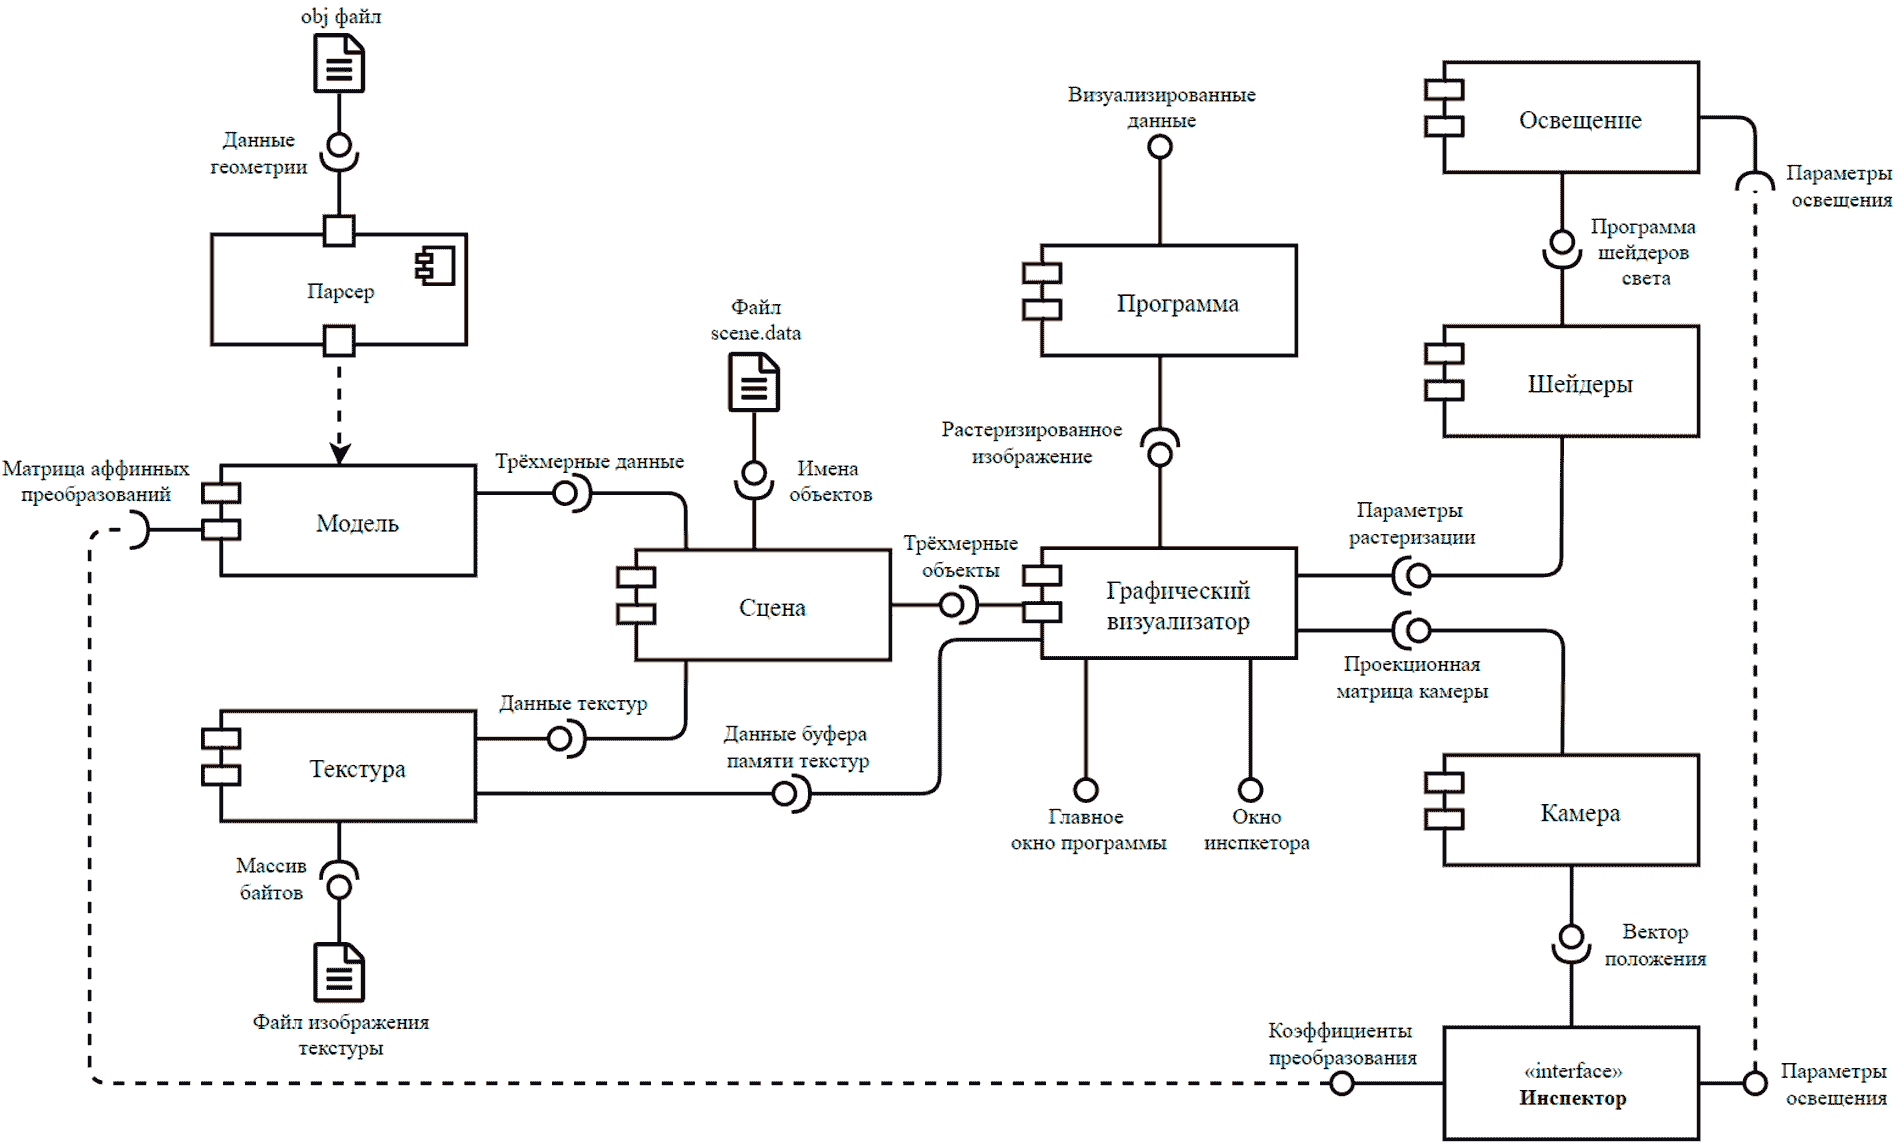
\includegraphics[width=1.025\linewidth]{diagram5.png}}
\caption{Диаграмма компонентов программы}
\label{diagram5:image}
\end{figure}

Данная диаграмма определяет общую архитектуру приложения, все его компоненты, а также устанавливает зависимости между ними в программной системе. Далее мы подробно опишем работу каждого компонента по отдельности.

\paragraph{Компонент Файл OBJ}

Является файлом с данными, расширения *.obj, содержащим данные трёхмерной геометрии объекта.

Предоставляет общий набор данных геометрии трёхмерной модели.

\paragraph{Компонент Парсер}

Синтаксический анализатор, преобразующий общий набор данных геометрии в отдельные массивы, подходящие по стандарту программной системы для корректной визуализации объектов.

Принимает общие данные геометрии трёхмерных моделей.

Является компонентом, зависимым от модуля Модель.

\paragraph{Компонент Модель}

Выполняет функцию обработки и хранения массивов трёхмерных данных. Преобразовывает, хранит и передаёт данные файла геометрии трёхмерного объекта.

Предоставляет массивы трёхмерных данных, понятных в интерпретации для программной среды.

\paragraph{Компонент Файл изображения текстуры}

Является файлом растрового изображения в форматах *.png или *.jpg.

Предоставляет закодированное изображение текстуры в виде массива байтов.

\paragraph{Компонент Текстура}

Обработчик изображения, который генерирует текстуру в системе и задаёт параметры для отрисовки и фильтрации изображения. Выделяет место в буффере текстур, а также привязывает ей определенный идентификатор в памяти буфера видеоадаптера.

Принимает массив байтов изображения текстуры.

Предоставляет общие данные текстуры в системе - её идентификатор и адрес в буфере памяти.

\paragraph{Компонент Файл scene.data}

Файл в который программа записывает и хранит данные идентификаторов, имён и ссылок на модели и текстуры.

Передаёт набор синтаксически размеченных строк, определяющих имена моделей и текстур.

\paragraph{Компонент Сцена}

Виртуальная сцена, которая представляет из себя словарь моделей и текстур, связывающий их идентификаторы в общую структуру объекта.

Принимает трёхмерные данные моделей, системы данные и параметры текстур, а также имён - идентификаторов моделей и текстур.

Передаёт обработанные и структурированные данные трёхмерных объектов, готовых к визуализации.

\paragraph{Компонент Инспектор}

Часть графического интерфейса программы, через который пользователь может производить взаимодействия над параметрами виртуальной среды и трёхмерными объектами, загруженными на виртуальную сцену.

Принимает данные вектора положения камеры.

Предоставляет коэффициенты для осуществления трансформации матриц аффинных преобразований. Также предоставляет параметры настройки освещения.

\paragraph{Компонент Камера}

Описывает матрицу перспективы, по которой происходит создание перспективы виртуальной среды.

Предоставляет проекционную матрицу перспективы.

\paragraph{Компонент Освещение}

Программа шейдера, отвечающая за обработку отражения света, а также уровня яркости грани модели, в зависимости от положения источника света.

Принимает параметры для настроек аттрибутов освещения.

Предоставляет программу шейдеров света.

\paragraph{Компонент Шейдеров}

Общая программа шейдеров, отвечающая за обработку отображения цвета и текстур вершин и граней моделей.

Принимает программу шейдеров света.

Предоставляет параметры шейдинга для финальной растеризации визуализированной сцены.

\paragraph{Модуль Графический визуализатор}

Главный блок программы, представляющий собой графический визуализатор, связывающий все модули программной среды, обрабатывая все необходимые данные для создания композиции и визуализации сцены трёхмерной среды.

Принимает обработанные массивы данных трёхмерных объектов, данные буфера памяти текстур, параметры программ шейдеров, а также матрицу проекции камеры.

Предоставляет графический интерфейс в виде главного окна программы и окна инспектора. Также передаёт конечное растрированное изображение в главный класс программы.

\paragraph{Компонент Программа}

Является начальным родительским компонентом всей программной среды, который осуществляет запуск приложения с определенными параметрами. Осуществляет запуск графического визуализатора с заданными аттрибутами.

Принимает данные графического визуализатора в виде растеризированного кадра.

Визуализирует растеризированную композицию кадра виртуальной сцены у пользователя на экране в главном окне программы.

\subsection{Описание файлов трёхмерных данных формата OBJ}
Формат файлов OBJ, или же Wavefront .obj файл - это формат файлов описания геометрии, разработанный в 1992 году компанией компьютерной графики Wavefront Technologies. Он содержит только 3D геометрию, а именно: позицию каждой вершины, связь координат текстуры с вершиной, направления нормалей, а также параметры, которые создают триангулярные примитивы. На основе файлов данного формата, завязан главный принцип работы разрабатываемой программной среды. 

Данный формат файла имеет следующие особенности:
\begin{itemize}
	\item он позволяет пользователям использовать файловое представление объектов сложной или неевклидовой формы, разделяя поверхность на треугольные грани, которые называются триангулярными примитивами. Данный процесс трасселяции упрощает процесс манипуляции, моделирования и визуализации, поскольку позволяет изменять каждую грань независимо от остальных;
	\item ещё одной важной особенностью является способность определять свойства поверхности трёхмерной геометрии объектов, такие как определение координат текстур и карты нормалей для шейдинга;
	\item OBJ поддерживает данные высокого разрешения, в сравнении со схожими форматами трёхмерных данных, к примеру, такими как STL;
	\item и в заключении, ещё одной особенностью данного формата является возможность хранения сразу нескольких текстур и цветов в одном объекте, в отличие от файлов, как в том же формате STL.
\end{itemize}

Несмотря на то, что данный формат расширения файлов используется уже более тридцати лет, он не является устаревшим, а даже более того - почти основным и универсальным форматом хранения данных трёхмерной геометрии. 

Существует множество способов открыть OBJ-файл и преобразовать его в различные другие форматы. Одним из вариантов является использование такого программного обеспечения, как 3DS Max, Solidworks, Cinema 4D или Blender, которое позволяет легко импортировать 3D-модели в формате OBJ, а затем преобразовывать и экспортировать их в любой необходимый формат.

Также данные объекта в OBJ-файле можно редактировать даже не запуская ни одно из программных обеспечений для трёхмерной графики, а просто открыв его в блокноте. Данный формат не закодирован какой-либо особой системой, и представлен в виде простого незашифрованного набора текста - данных трёхмерной геометрии. Пример содержания OBJ-файла представлен в ПРИЛОЖЕНИИ А.

\subsection{Описание работы парсера}

В результате необходимости импортирования и использования в программной среде файлов трёхмерных данных с расширением *.obj из внешней файловой системы устройства, возникла необходимость автоматизировать загрузку и интерпретацию этих данных для программы. Для решения данной задачи был разработан специальный алгоритм программы парсера.

Парсер, или же синтаксический анализатор - часть программы, которая преобразовывает текстовые входные данные в структурированный формат.

Исходя из этого, необходимо, чтобы парсер мог разделить все эти данные на отдельные массивы, которые будет использовать программа. В заключение вышесказанного, можно построить схему, по которой должен будет работать парсер, как показано на рис.~\ref{diagram4:image}, где изображена схема работы подпрограммы парсера.

\begin{figure}[ht]
	\center{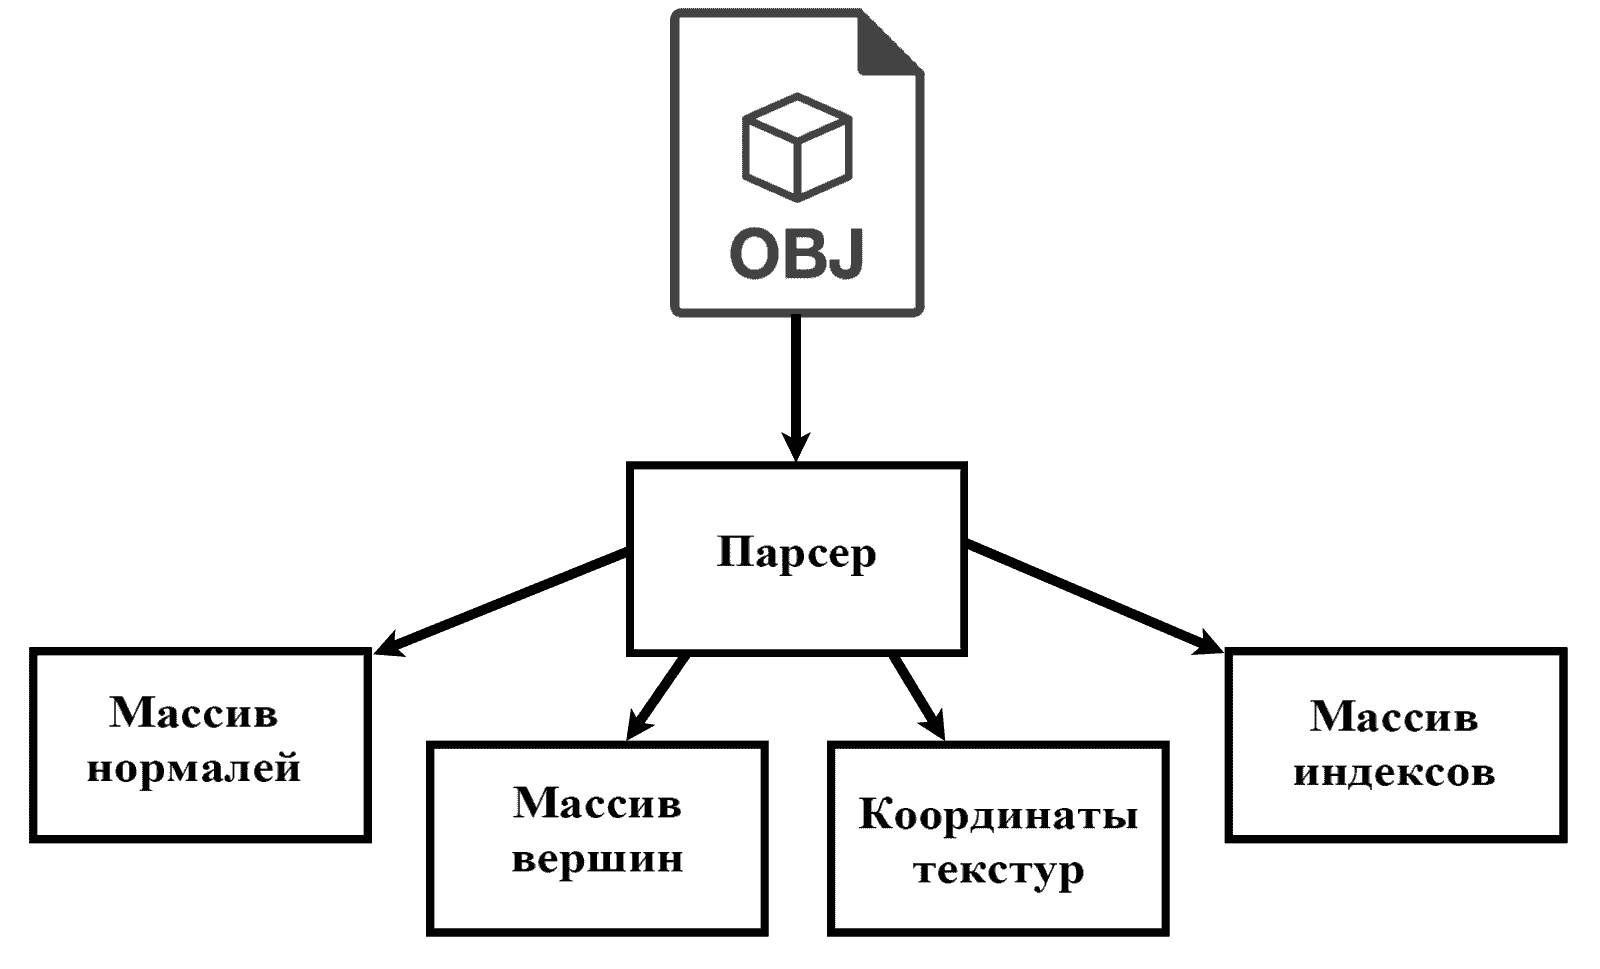
\includegraphics[width=1\linewidth]{diagram4.png}}
	\caption{Схема работы программы парсера}
	\label{diagram4:image}
\end{figure}

На данной схеме показано, на какие массивы данных разбивается OBJ-файл в результате синтаксического анализа парсера. Данные массивы необходимо будет использовать по отдельности, чтобы каждый был задействован в соответствующих модулях и подпрограммах программной среды.

Парсер не представляет собой отдельный независимый класс. Он является компонентом модуля, и его подпрограмма находится в классе Model. Это создаёт удобство в использовании данного класса, так как в следствии, каждый его элемент будет иметь возможность автоматически интерпретировать и структурировать данные геометрии своей модели в массивы трёхмерных данных, в результате чего, они сразу смогут структурироваться под стандарты программы, при инициализации элемента класса Model.

Фрагмент листинга кода парсера представлен в ПРИЛОЖЕНИИ Г.

\subsection{Система хранения данных внутри проекта}

Программная система имеет начальный набор данных - текстуры и файлы геометрии, чтобы пользователь мог начать ознакомление с программой со встроенных данных, без необходимости подгружать дополнительные файлы из системы для полноценной работы программы. В ситуации, в которой количество хранимых файлов приложением больше одного, возникла необходимость спроектировать структурированную систему индексирования и хранения всех данных, чтобы программа понимала, какие данные в текущий момент пользователь планирует использовать.
Для того, чтобы приложение могло работать с большим количеством данных и файлов, была разработана система хранения данных, которая имеет свои принципы и особенности. К файлам проекта программная система обращается через два файла данных - "<Objects.data"> и "<Resources.data">.

\subsubsection{Файл Resource.data}

В файле "<Resources.data"> программа записывает и считывает массив всех хранимых программой ресурсов - файлов геометрии и текстур. Каждая строка представляет собой отдельный ресурс - либо файл геометрии, либо текстуры, в которой записано их имя - относительный путь к файлам внутри проекта. Хранение ресурсов осуществляется по принципу листа, который проще говоря, является динамически расширяемым массивом данных, который можно расширять с конца. Данные ресурсы используются для дальнейшего представления объектов. Пример содержания и синтаксиса файла приведён в ПРИЛОЖЕНИИ В.

\subsubsection{Файл Objects.data}

В файле "<Objects.data"> программа записывает и считывает структуру объекта. Каждая строка файла представляет собой отдельный объект, который состоит из трёх частей - имени объекта, файла геометрии OBJ и файла изображения текстуры. Хранение объектов осуществляется по принципу словаря, где к каждому имени объекта привязаны свои определенные модели и текстуры, что собственно и является самими представлением объекта. Пример содержания и синтаксиса файла приведён в ПРИЛОЖЕНИИ В.

\subsection{Проектирование пользовательского интерфейса}

Графический прототип интерфейса, показанный на рис.~\ref{maket2:image} демонстрирует, какие элементы пользовательского интерфейса будут включены в конечную реализацию программы.

\begin{figure}[H]
\center{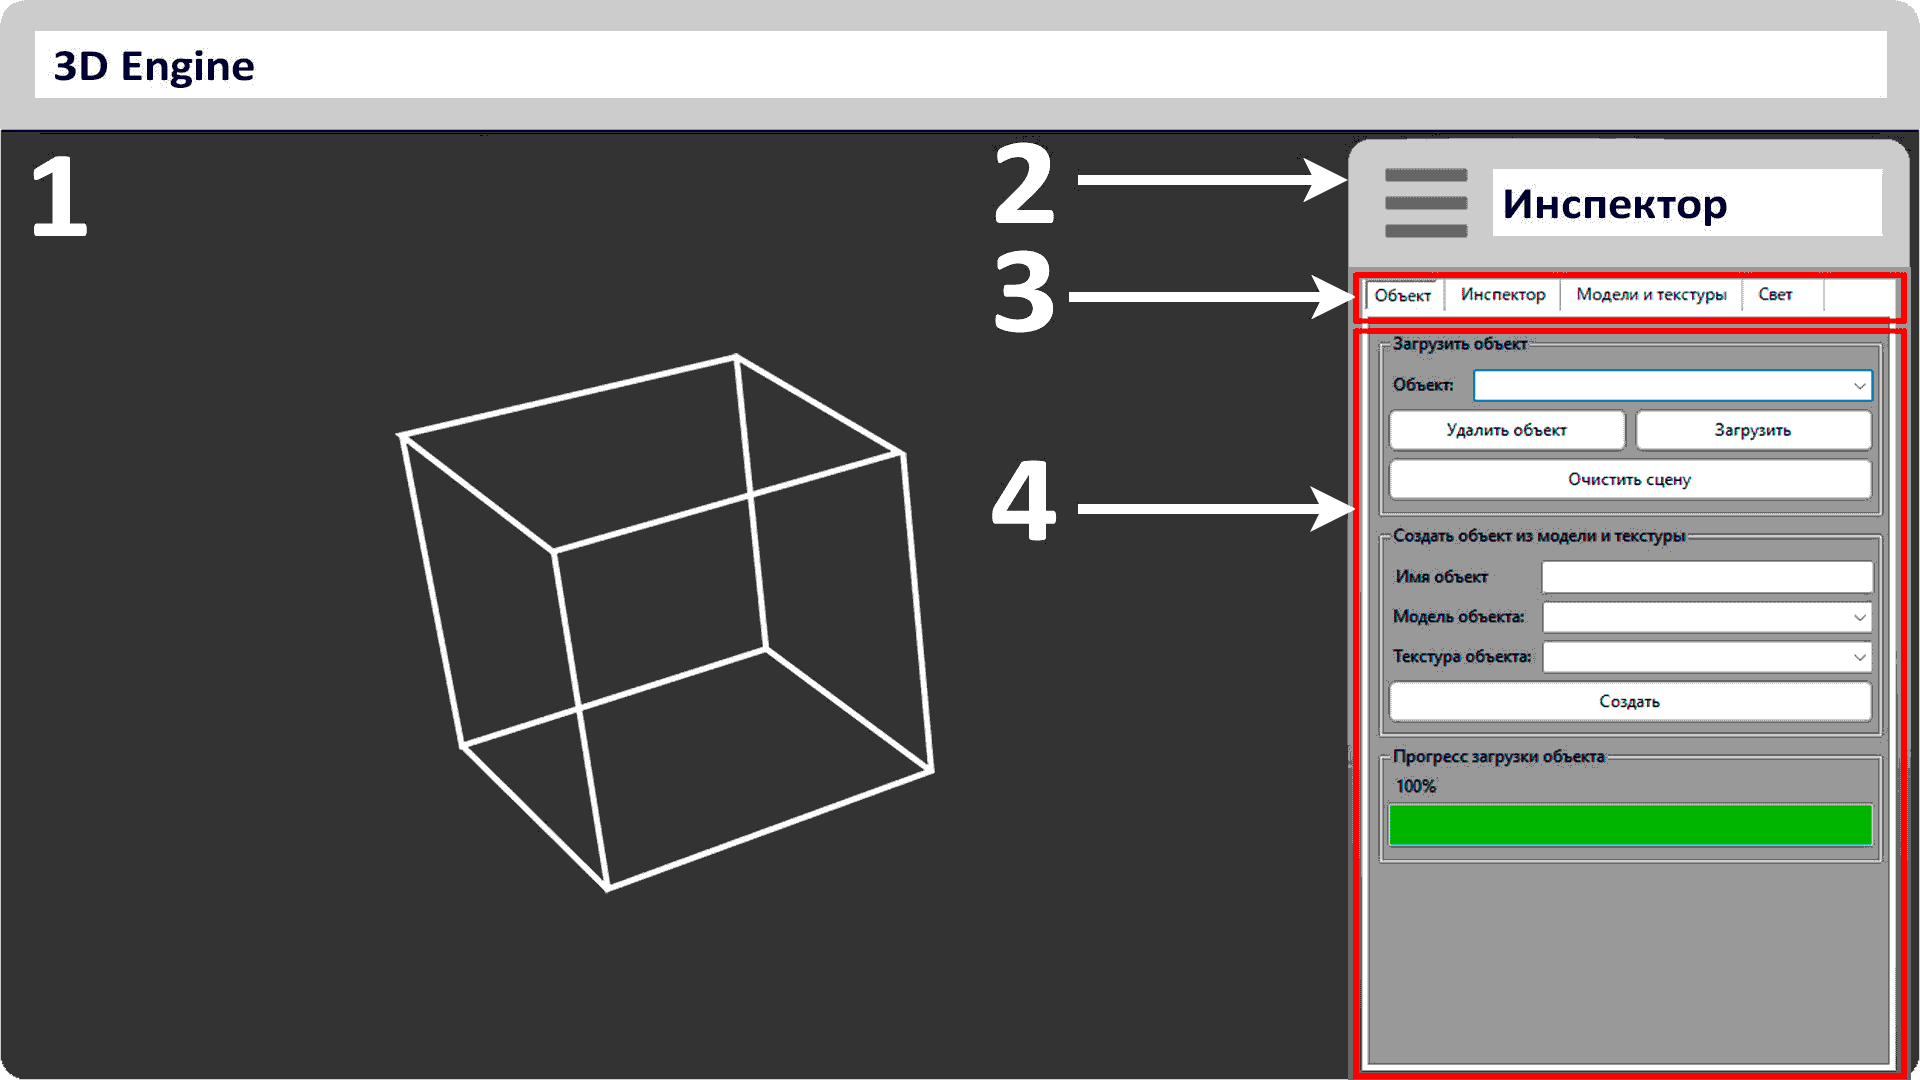
\includegraphics[width=1\linewidth]{maket2.png}}
\caption{Прототип пользовательского интерфейса}
\label{maket2:image}
\end{figure}

Описание элементов интерфейса, показанного на рис.~\ref{maket2:image}:
\begin{enumerate}
	\item Главное окно программы. Выводит визуализированные данные на экран.
	\item Окно инспектора.
	\item Вкладки окон инспектора.
	\item Активное меню вкладки инспектора.
\end{enumerate}

\subsubsection{Главное окно программы}

Главное окно программы представляет из себя виртуальную трёхмерную среду с одноцветным фоном. Оно служит для отображения визуализации трёхмерных моделей, которые пользователь загрузит в программу. Также данное окно является частью пользовательского интерфейса с интуитивной функцией ввода - пользователь может управлять направлением перспективы взгляда камеры, зажав правую кнопку мыши и направляя курсор в нужную сторону, чтобы управлять камерой и осматриваться в виртуальном пространстве. А используя колесо прокрутки, пользователь может отдалять и приближать угол обзора.

Управление перемещением камеры в пространстве также осуществляется в главном окне программы, с помощью клавиатуры:
\begin{itemize}
	\item клавиша «W» – переместить камеру вперёд по направлению взгляда;
	\item клавиша «A» – переместить камеру вправо относительно направления взгляда;
	\item клавиша «S» – переместить камеру назад по направлению взгляда;
	\item клавиша «D» – переместить камеру влево относительно направления взгляда;
	\item клавиша «левый Shift» – поднять камеру вверх, по координате +Y;
	\item клавиша «левый Ctrl» – опустить камеру вниз, по координате -Y;
\end{itemize}

\subsubsection{Окно инспектора}

Инспектор - это дополнительное окно, расположенное по краю справа, поверх главного окна. Оно служит вспомогательным элементом интерфейса, чтобы пользователь мог взаимодействовать и управлять элементами внутри виртуальной сцены. Например, выполнять преобразование массива данных трёхмерной модели - перемещать её в пространстве, наклонять под определённым углом и прозводить растяжение или сжатие, и всё это по всем трём координатам.

\subsubsection{Вкладки окон инспектора}

Меню со вкладками окон инспектора, где пользователь может выбрать одну трёх вкладок, чтобы переключать и менять содержание активного меню инспектора.

\subsubsection{Активное меню вкладки инспектора}

Показывает основной интерфейс меню инспектора. Инспектор имеет три разных активных меню, и содержание окна инспектора будет меняться, в зависимости от выбранной вкладки.

\paragraph{Вкладка "<Объект">}
Вкладка "<Объект"> - в данной вкладке пользователь может выбрать из выпадающего списка объект, который он хочет загрузить и визуализировать на виртуальной сцене. Также данная вкладка имеет ещё один важный раздел, в котором пользователь может создать новый объект внутри проекта - связав выбранный файл из списка моделей и файл из списка текстур, имеющихся внутри проекта, в новую сущность, дав имя получившемуся объекту.

\paragraph{Вкладка "<Инспектор">}
Вкладка "<Инспектор"> - это информационная вкладка, в которой показаны точные координаты и наклон камеры, а также в которой пользователь может осуществить аффиинные преобразования над загруженной моделью на сцену в данный момент и узнать данные об уже раннее произведенных преобразованиях над моделью: смещении, наклона и масштабировании.

\paragraph{Вкладка "<Модели и текстуры">}
Вкладка "<Модели и текстуры"> содержит весь список доступных моделей и текстур в программе, загруженных пользователем. Также в ней пользователь может осуществлять непосредственно саму загрузку массивов трёхмерных данных с расширением *.obj в программу и изображений текстур с расширением *.png и *.jpg. Также в данной вкладке пользователь может удалить уже существующие файлы моделей и текстур из проекта.

\paragraph{Вкладка "<Свет">}
Во вкладке "<Свет"> пользователю представлены текущие настройки параметров всех типов освещений, излучаемых источником света, которые пользователь может свободно изменять, чтобы получить желаемый результат отрисовки освещения отраженного и рассеянного света то поверхности объекта.
\ifПрактика{}\else{
   \section{Рабочий проект}
\subsection{Классы, использованные при разработке программной системы}

В результате разработке программной системы было спроектировано множество классов и методов, которые продемонстрированы в таблице \ref{class:table}).

\renewcommand{\arraystretch}{0.8} % уменьшение расстояний до сетки таблицы
\begin{xltabular}{\textwidth}{|X|p{6.5cm}|>{\setlength{\baselineskip}{0.7\baselineskip}}p{6.25cm}|>{\setlength{\baselineskip}{0.7\baselineskip}}p{3.85cm}|}
\caption{Описание классов, используемых в приложении\label{class:table}}\\
\hline \centrow \setlength{\baselineskip}{0.7\baselineskip} Название класса & \centrow Описание класса & \centrow Методы \\
\hline \centrow 1 & \centrow 2 & \centrow 3\\ \hline
\endfirsthead
\caption*{Продолжение таблицы \ref{class:table}}\\
\hline \centrow 1 & \centrow 3 & \centrow 4\\ \hline
\finishhead
Engine & Engine – класс программы, представляющий собой графический визуализатор, связывающий между собой основные модули и классы программной среды, обрабатывая все необходимые данные для создания композиции и визуализации сцены трёхмерной среды. &
\textbf{void Run\_Inspector()}
	
Запускает окно Инспектора

\textbf{void OnLoad()}
	
Событие, вызываемое при полной загрузке программы, определяющее первоначальную визуализацию пустой сцены

\textbf{void Initialize()}
	
Метод инициализации и отрисовки объектов на виртуальной сцене

\textbf{void OnRenderFrame(Fr- ame EventArgs e)}
	
Событие, вызываемое каждый раз при создании нового кадра приложением

\textbf{void OnUpdateFrame(Frame- EventArgs e)}
	
Событие, вызываемое каждый раз при изменении или обновлении кадра пользователем\\

\hline & & 
\textbf{void ReloadScene()}
	
Метод, перезагружающий виртуальную сцену, перерисовывая заново все объекты на сцене
	
\textbf{void OnMouseWheel(Mouse- WheelEventArgs e)}
	
Событие, вызываемое при прокрутке колеса мыши

\textbf{void OnResize(ResizeEventArgs e)}
	
Событие, вызываемое при изменении размера окна приложения

\textbf{void OnClosing(CancelEventArgs e)}
	
Событие, вызываемое при закрытии главного окна приложения

\textbf{OnInspectorClose(object sender, EventArgs e)}
	
Событие, вызываемое при закрытии окна инспектора\\
\hline Program & Program – главный класс программы, который задаёт настройки и запускает класс графического визуализатора & 
\textbf{void Main()}
	
Главный метод программы\\
\hline Scene & Класс Scene выполняет роль хранилища моделей и изображений, а также выполняет роль виртуальной сцены, на которой находятся все трёхмерные объекты и остальные элементы, участвующие в визуализации. При инициализации выполняет загрузку объектов и привязанных к ним данных массивов моделей и файлов текстур, которые уже были раннее загружены в проект &

\textbf{public Scene()}
	
Метод инициализации класса Scene

\textbf{void CreateObject(string name, string model\_name, string texture\_name)}
	
Метод создания нового объекта с указанным именем и выбранными данными трёхмерной модели и изображением текстуры
	
\textbf{void DeleteObject(string name)}
	
Метод удаления объекта с указанным именем

\textbf{List<string> DeleteRelatedObjects(string relate)}
	
Метод удаления объекта, который имеет содержит в себе вхождение файла relate. Возвращает лист имён удаленных объектов
	
\textbf{bool AddResourceModel(string origFile)}
	
Метод добавления ресурса нового файла модели в проект. Возвращает bool переменную, отображающую успешность выполнения добавления нового или перезаписи существующего файла в проекте\\
\hline &  & 
\textbf{bool AddResourceTexture(string origFile)}

Метод добавления ресурса нового файла изображения текстуры в проект. Возвращает bool переменную, отображающую успешность выполнения операции добавления нового или перезаписи существующего файла в проекте

\textbf{void RemoveResource(string resName, string type)}

Метод удаления указанного файла ресурса из проекта

\textbf{string GetFileName(string origFile) }

Метод, возвращающий имя файла из указанного полного пути

\\
\hline Model & Model - класс, описывающий трёхмерную модель объектов. Выполняет роль приёма, хранения и передачи массива трёхмерных данных для обработчика триангулярных примитивов. При создании выполняет чтение и преобразование в массивы вершин и индексов, загруженного файла с данными трёхмерного объекта &
\textbf{public Model(string path)}

Метод, инициализирующий новый класс Model, используя файл трёхмерных данных по указанному пути

\textbf{float[] GetVertices()}

Метод, возвращающий массив вершин объекта, в данный момент загруженного и обработанного классом Model

\textbf{uint[] GetIndices()}

Метод, возвращающий массив индексов объекта, в данный момент загруженного и обработанного классом Model
\\
\hline Shader & Shader - класс, представляющий программу настройки конечной визуализации, и при инициализации создаёт подпрограмму в общей графике, для преобразования растеризированного изображения внутри буффера памяти видеоадаптера, для отображения текстур и освещения &
\textbf{Shader(string vertPath, string fragPath)}

Метод инициализации нового элемента класса Shader, используя программы шейдеров вершин и фрагментов по указанным путям

\textbf{void CompileShader(int shader)}

Метод компиляции указанного шейдера

\textbf{void LinkProgram(int program)}

Внутренний метод, связывающий объект программы шейдеров с указанной переменной

\textbf{void Use()}

Метод активации раннее связанной программы шейдера

\textbf{int GetAttribLocation(string attribName)}

Метод, возвращающий местонахождения указанного атрибута в шаблоне программы шейдера
\\
\hline Texture & Texture - класс описывающий данные, параметры и атрибуты текстуры изображения. При инициализации выделяет место в буффере памяти видеоадаптера для загруженной в программу текстуры, а также обрабатывает настройки параметров её отображения &
\textbf{Texture LoadFromFile(string path)}

Метод, инициализирующий текстуру из файла

\textbf{void Use(TextureUnit unit)}

Метод, указывающий, какая текстура будет использоваться в проекте
\\
\hline Inspector & Класс Inspector - является частью пользовательского интерфейса, представляющего из себя окно взаимодействия между пользователем и программой. Служит для того, чтобы пользователь осуществлял загрузку собственных массивов трёхмерных данных моделей и текстур в проект, а также осуществлял указанные аффинные преобразования над загруженными моделями. & 
\textbf{public Inspector()}

Метод инициализации инспектора

\textbf{void Inspector\_Load(object sender, EventArgs e)}

Событие, срабатывающее по окончании загрузки инспектора

\textbf{void timer1\_Tick(object sender, EventArgs e)}

Событие, срабатывающее каждый тик таймера

\textbf{void openFileModel\_Ok(object sender, CancelEventArgs e)}

Событие, срабатывающее при подтверждении выбора файла модели

\textbf{void openFileTexture\_Ok(object sender, CancelEventArgs e)}

Событие, срабатывающее при подтверждении выбора файла текстуры

\textbf{void trackBar\_colorRed\_Scroll (object sender, EventArgs e)}

Метод обработчика скроллбара красного цвета

\textbf{void trackBar\_colorGreen\_Scroll (object sender, EventArgs e)}

Метод обработчика скроллбара зеленого цвета

\textbf{void trackBar\_colorBlue\_Scroll (object sender, EventArgs e)}

Метод обработчика скроллбара синего цвета
\\
\hline Camera & Класс Camera представляет собой матрицу преобразования, которая служит для корректного отображения перспективы виртуального трёхмерного вида сцены, и для того, чтобы конечный вид проекции сцены был перспективным, а не ортографическим &
\textbf{Camera(Vector3 position, float aspectRatio)}

Метод инициализации камеры

\textbf{Matrix4 GetViewMatrix()}

Метод, возвращающий текущую матрицу взгляда камеры

\textbf{Matrix4 GetProjectionMatrix()}

Метод, возвращающий текущую матрицу проекции камеры

\textbf{void UpdateVectors()}

Метод, обновляющий координаты и векторы камеры
\end{xltabular}
\renewcommand{\arraystretch}{1.0} % восстановление сетки

\subsection{Системное тестирование разработанной программной системы}

В соответствии с реализованными функциями программы, было разработано специализированное системное тестирование, подходящее для тестирования данного программного продукта, которое включает себя набор тестовых случаев, чтобы проверить работоспособность всех осуществляемых функций программы.

\subsubsection{Тестовый случай: Инициализация ресурсов программы}
Действия пользователя: Пользователь запускает программу.

Ожидаемый результат: Открывается два окна программы. Окно инспектора должно быть поверх всех окон. Программа загружает ресурсы из указанного во внутренних файлах данных пути проекта, и все загруженные ресурсы должны корректно отображаться в проекте.

Ход выполнения:

При запуске программы на экране пользователя отображаются два окна: главное окно вывода и окно инспектора. Окно инспектора находится поверх всех окон, как показано на рисунке ~\ref{screen1:image}.

\begin{figure}[H]
	\center{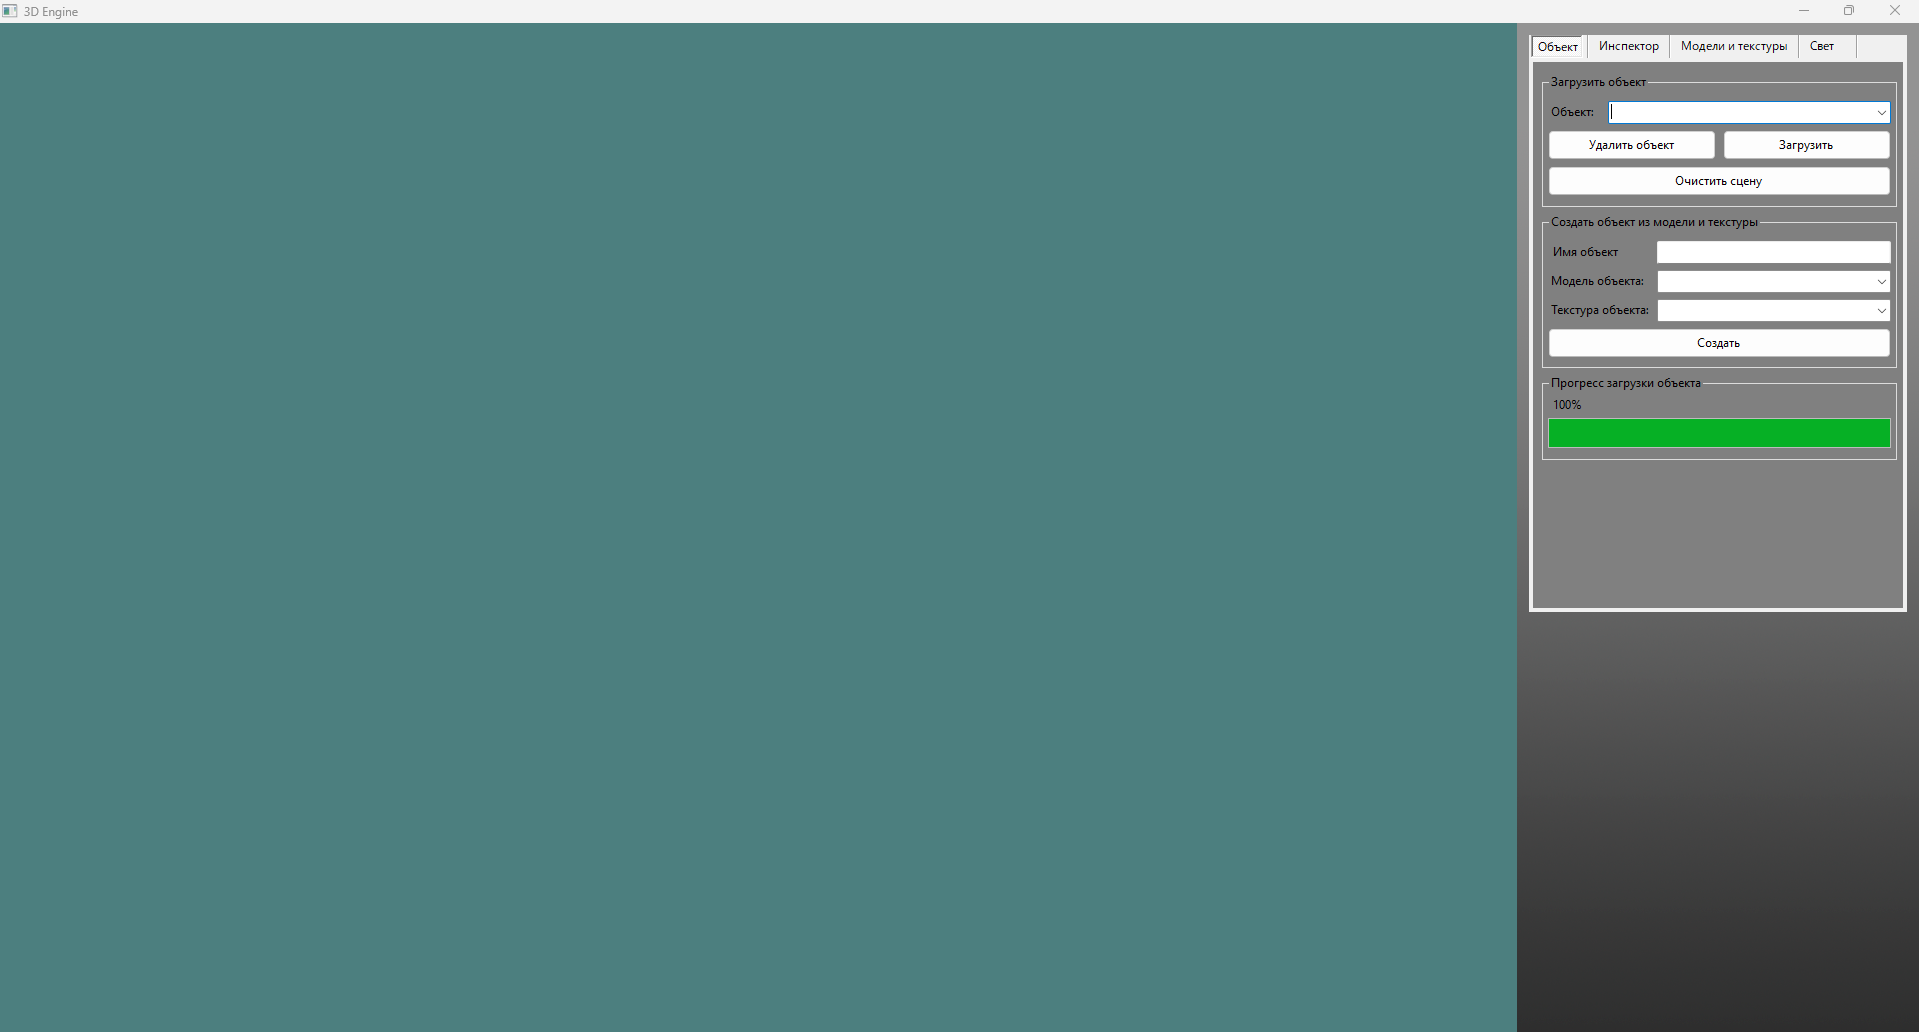
\includegraphics[width=1\linewidth]{screen1.png}}
	\caption{Интерфейс программы с двумя окнами}
	\label{screen1:image}
\end{figure}

Далее необходимо убедиться, что все объекты и данные ресурсов, которые указаны в примере файлов Resources.data и Objects.data в ПРИЛОЖЕНИИ В, были интерпретированы и загружены в программу.

При нажатии на контекстное меню напротив надписи "<Объект">, появляется выпадающий список, как показано на рисунке ~\ref{screen2:image}, содержащий все загруженные программой объекты, указанные в файле Objects.data.

\begin{figure}[H]
	\center{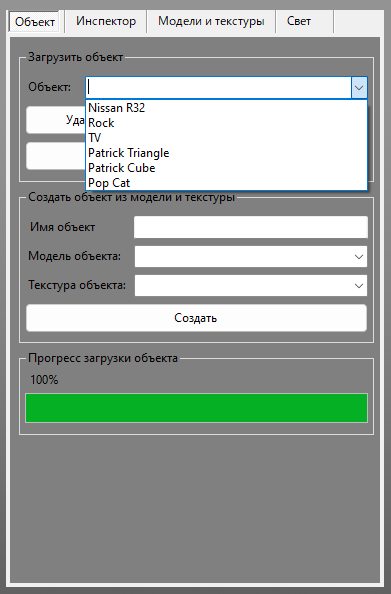
\includegraphics[width=0.6\linewidth]{screen2.png}}
	\caption{Объекты, инициализированные программой}
	\label{screen2:image}
\end{figure}

При нажатии на контекстное меню напротив надписей "<Модель объекта"> и "<Текстура объектов">, появляются выпадающие списки, содержащие ресурсы, загруженные программой при запуске, как показано на рисунках ~\ref{screen3:image} и ~\ref{screen4:image}.

\begin{figure}[H]
	\center{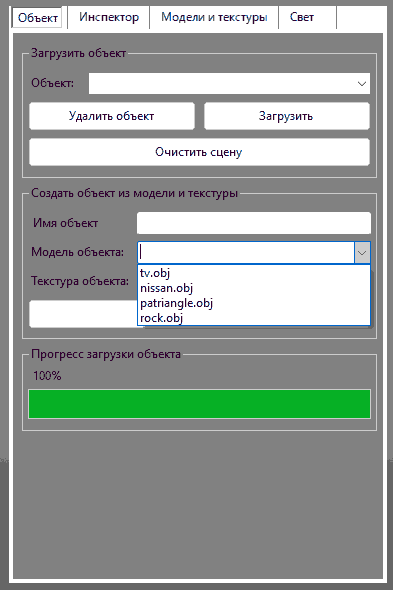
\includegraphics[width=0.6\linewidth]{screen3.png}}
	\caption{Список моделей, загруженныз в проект}
	\label{screen3:image}
\end{figure}

\begin{figure}[H]
	\center{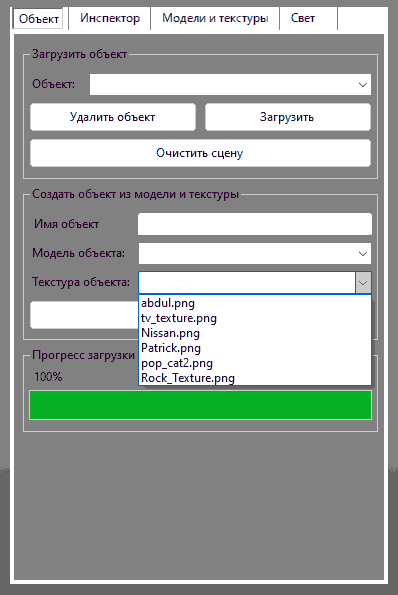
\includegraphics[width=0.6\linewidth]{screen4.png}}
	\caption{Список текстур, загруженных в проект}
	\label{screen4:image}
\end{figure}

На данных изображениях видно, что программа успешно загрузила все объекты и ресурсы, которые были указаны в файлах хранения данных.

\subsubsection{Тестовый случай: Визуализация объекта на сцене}
Действия пользователя: Пользователь пытается загрузить выбранный объект из выпадающего списка объектов на виртуальную сцену.

Ожидаемый результат: Выбранный пользователем объект корректно отображается на виртуальной сцене в главном окне программы.

Ход выполнения:

В открывшемся окне инспектора, пользователь открывает выпадающий список объектов, и выбирает строку с желаемым именем объектом. После чего, нажимает на кнопку "<Загрузить"> и запускается процесс отрисовки трёхмерного объекта. Прогресс визуализации можно наблюдать по шкале прогресса в окне инспектора чуть ниже, в разделе "<Прогресс загрузки">.

\begin{figure}[H]
	\center{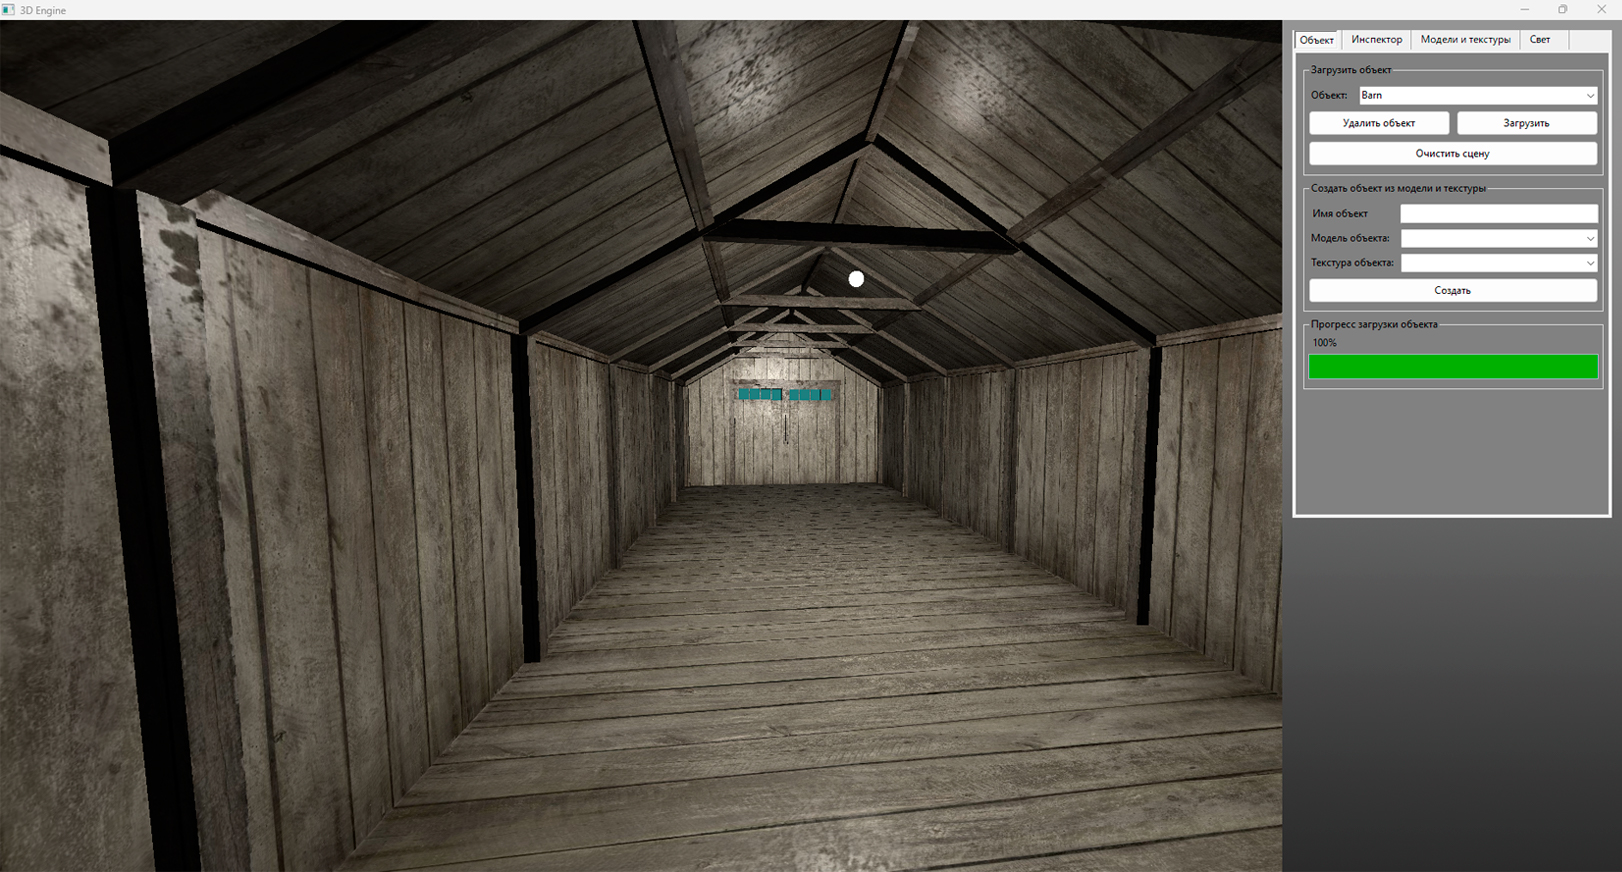
\includegraphics[width=1\linewidth]{screen15.jpg}}
	\caption{Главное окно программы с корректно отрисованным объектом на сцене}
	\label{screen15:image}
\end{figure}

После окончания визуализации объекта, пользователь увидит его в главном окне программы и сможет управлять перемещением камеры, настройкой света и выполнять трансформации над загруженным объектом.

\subsubsection{Тестовый случай: Настройка освещения}
Действия пользователя: Пользователь изменяет параметры источника света: цвет освещения - пытается ввести некорректные значения цвета в HEX формате, интенсивность общего света, интенсивность рассеянного света, интенсивность отраженного света и интенсивность отражения цвета.

Ожидаемый результат: Некорректные значения цвета в HEX формате преобразовываются в нейтрально белый цвет по умолчанию, источник света изменяет свои параметры в соответствии с веденными пользователем значениями.

Ход работы:

Для того, чтобы редактировать параметры света, необходимо, чтобы на сцене был загружен какой-либо объект, в противном случае изменение параметров света не будет иметь значения, так как не будет поверхностей, от которых свет мог бы отражаться.

В запущенной программе, пользователь переходит на вкладку инспектора "<Свет">. В открытой вкладке пользователь пытается ввести некорректные значения света в HEX-формате, как показано на рисунке ~\ref{screen17:image}. 

\begin{figure}[H]
	\center{
\includegraphics[width=0.7\linewidth]{screen17.png}}
	\caption{Пример некорректно введённого значения цвета в формате HEX}
	\label{screen17:image}
\end{figure}

После попытки применить данный некорректно введенный цвет к освещению, нажав на кнопку "<Выбрать цвет">, программа преобразует его в нейтрально белый цвет по умолчанию, как показано на рисунке ~\ref{screen18:image}.

\begin{figure}[H]
	\center{
\includegraphics[width=0.7\linewidth]{screen18.png}}
	\caption{Результат преобразования некорректного значения цвета HEX в нейтрально белый цвет}
	\label{screen18:image}
\end{figure}

Далее пользователь вводит остальные значения света, как в примере на рисунке ~\ref{screen16:image}.

\begin{figure}[H]
	\center{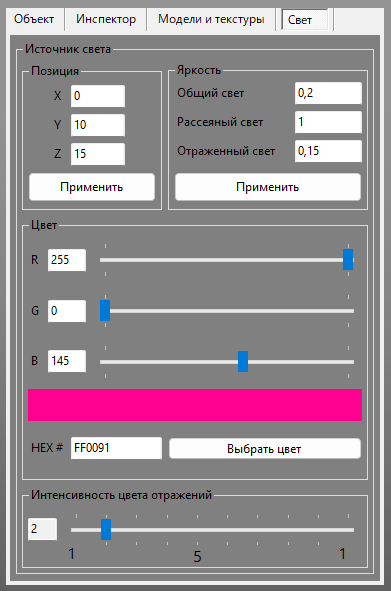
\includegraphics[width=0.6\linewidth]{screen16.png}}
	\caption{Пример введёных значений параметров света}
	\label{screen16:image}
\end{figure}

По мере введения данных значений, пользователь уже начнёт замечать изменения освещения. Ползунки, отвечающие за интенсивность одного из трёх цветов, применяют изменения к освещению сразу же, как только пользователь начал взаимодействовать с данным элементом интерфейса. Также моментально применяет свои значения и ползунок интенсивности отражения цвета.

Для применения изменения позиции и интенсивности света, необходимо нажать на кнопки "<Применить"> в соответствующих разделах поля.

Результат конечных изменений параметров света показан на рисунке ~\ref{screen19:image}.

\begin{figure}[H]
	\center{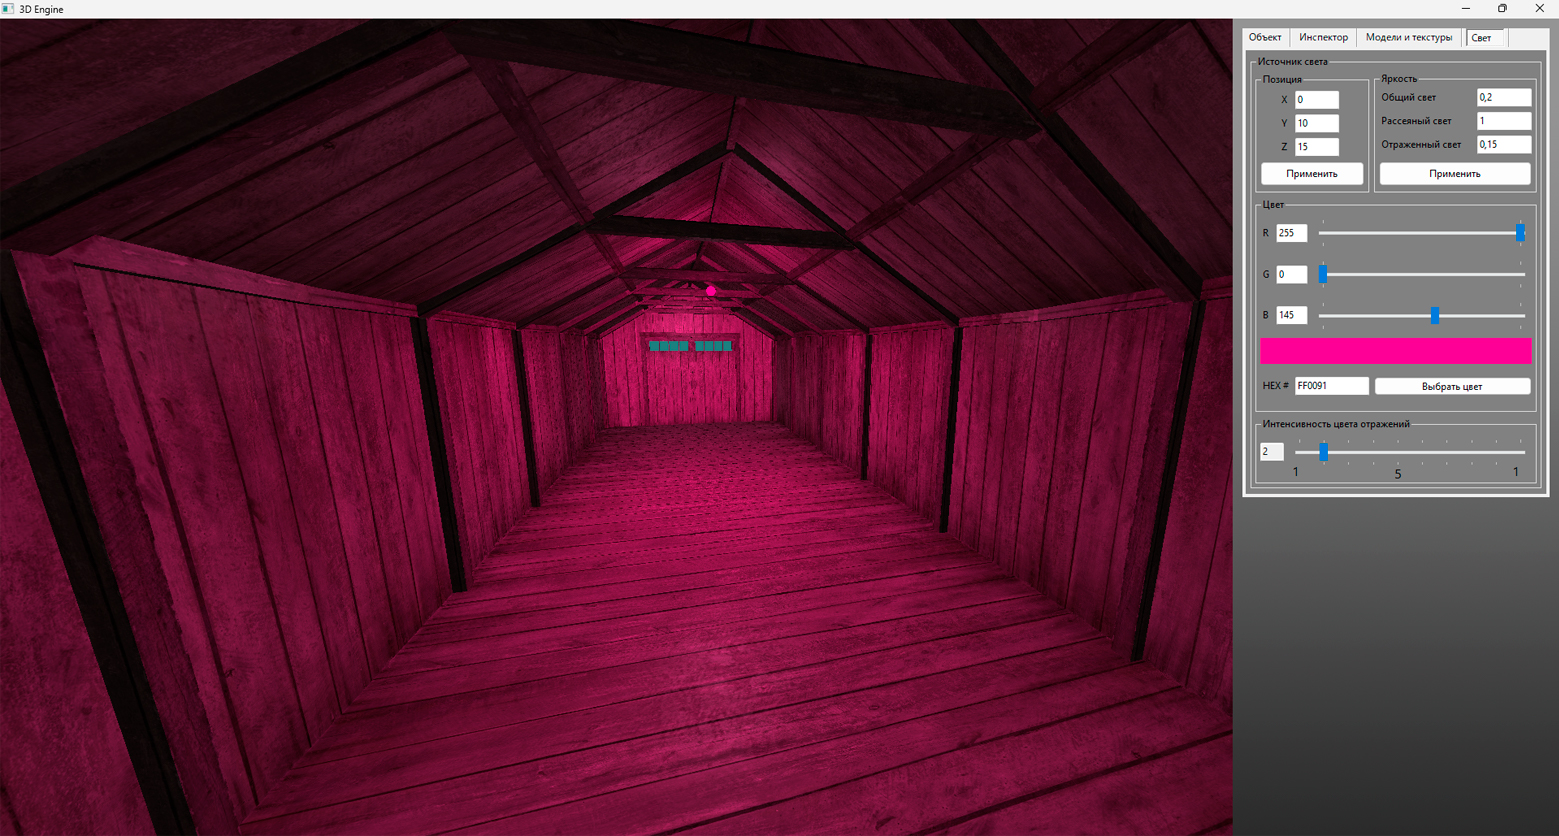
\includegraphics[width=1\linewidth]{screen19.jpg}}
	\caption{Результат изменений параметров света на виртуальной сцене}
	\label{screen19:image}
\end{figure}

\subsubsection{Тестовый случай: Трансформация объекта}
Действия пользователя: Пользователь загружает объект и пытается применить к нему трансформацию, вводя различные значения, включая отрицательные и значения, равные нулю.

Ожидаемый результат: Модель объекта, загруженного на сцену будет трансформирована, соответственно введенным пользователем значениям.

Ход выполнения:

Пользователь загружает объект на сцену, затем перейдя во вкладку "<Инспектор">, вводит значения трансформации модели объекта в соответствующие строки, как показано в примере на рисунке ~\ref{screen20:image}.

\begin{figure}[H]
	\center{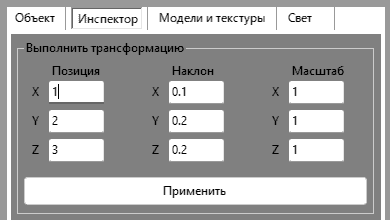
\includegraphics[width=0.6\linewidth]{screen20.png}}
	\caption{Пример введенных значений трансформации модели}
	\label{screen20:image}
\end{figure}

Чтобы применить данные трансформации, пользователь нажимает на кнопку "<Применить">. И результат становится виден на экране, как показано на рисунке ~\ref{screen21:image}.

\begin{figure}[H]
	\center{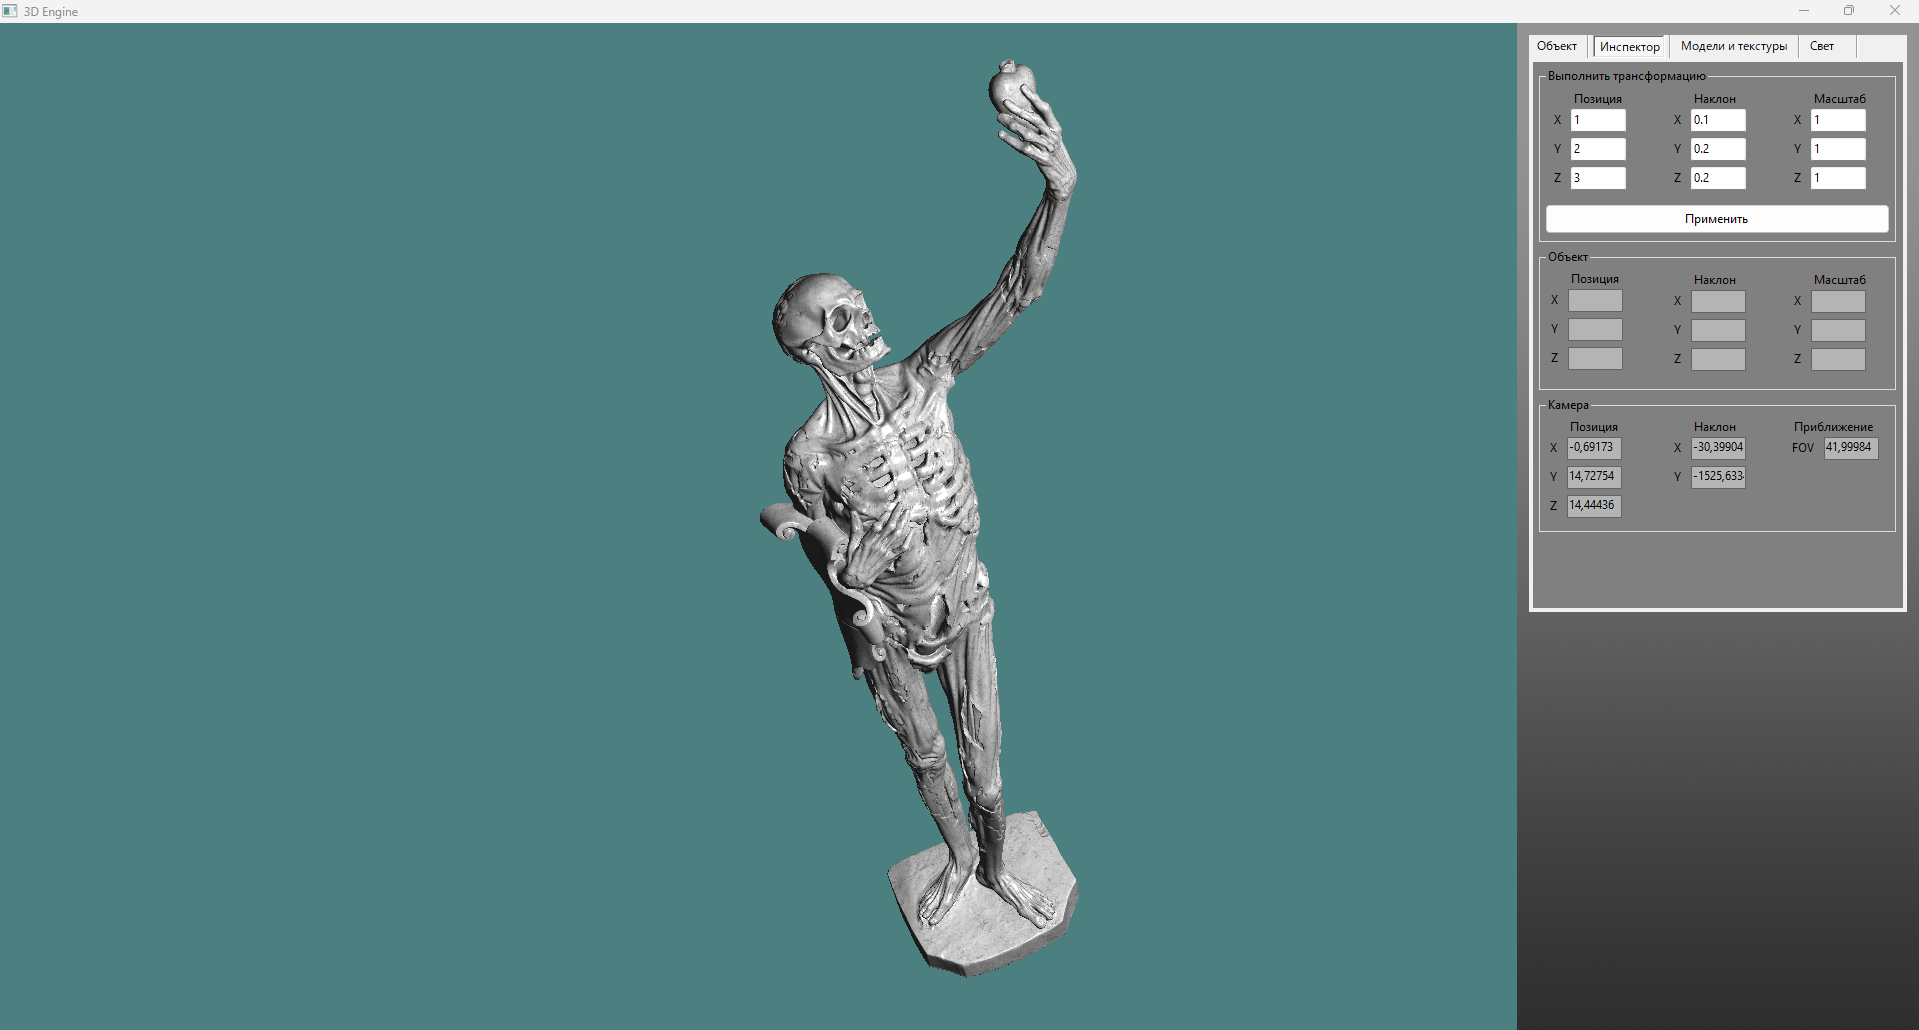
\includegraphics[width=1\linewidth]{screen21.png}}
	\caption{Результат трансформации трёхмерной модели объекта}
	\label{screen21:image}
\end{figure}

Как видно на снимке экрана, модель наклонилась набок, по осям в определенных значениях, указанным пользователем.

Все значения трансформаций, кроме значений масштаба модели могут быть равны нулю и отрицательными. Но в данном случае пользователь пытается задать нулевые значения для трансформации масштаба модели, как показано на рисунке ~\ref{screen22:image}

\begin{figure}[H]
	\center{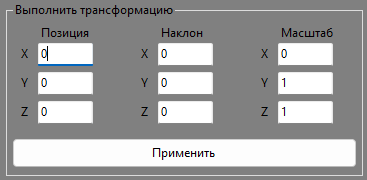
\includegraphics[width=0.6\linewidth]{screen22.png}}
	\caption{Трансформация масштаба, равная нулю в одной из координат}
	\label{screen22:image}
\end{figure}

Трансформация масштаба - это коэффициент матрицы, проще говоря число, на которое будет умножена матрица трёхмерной модели. Соответственно, при умножении матрицы на ноль, модель объекта по своей сути умножается на ноль и перестаёт существовать, так что пользователь будет наблюдать пустую виртуальную сцену.

\subsubsection{Тестовый случай: Импортирование ресурсов в проект}
Действия пользователя: Пользователь пытается загрузить собственные файлы моделей или текстур в проект со своего устройства, для дальнейшей работы с ними.

Ожидаемый результат: Файлы будут успешно загружены в проект, а пользователь сможет с ними взаимодействовать внутри программы.

Ход выполнения:

В открытой программе пользователь, переключившись на окно Инспектора, переходит во вкладку "<Модели и текстуры">, как показано на рисунке ~\ref{screen5:image}.

\begin{figure}[H]
	\center{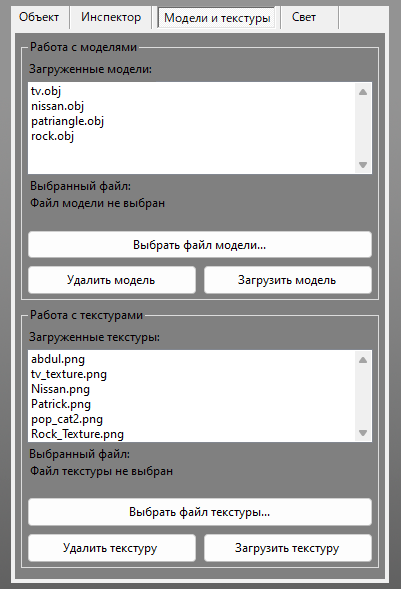
\includegraphics[width=0.6\linewidth]{screen5.png}}
	\caption{Открытая вкладка инспектора "<Модели и текстуры">}
	\label{screen5:image}
\end{figure}

На активном окне вкладки "<Модели и текстуры"> пользователь может видеть списки моделей и текстур, уже загруженные в проект. В зависимости от типа загружаемого файла в проект, пользователь нажимает на соответствующую кнопку. В данном случае пользователь желает загрузить файл трёхмерной модели объекта, и нажимает на кнопку "<Загрузить модель">. На экране появляется новое диалоговое окно с функцией выбора файла из системы устройства пользователя. Данное окно показано на рисунке ~\ref{screen6:image}.

\begin{figure}[H]
	\center{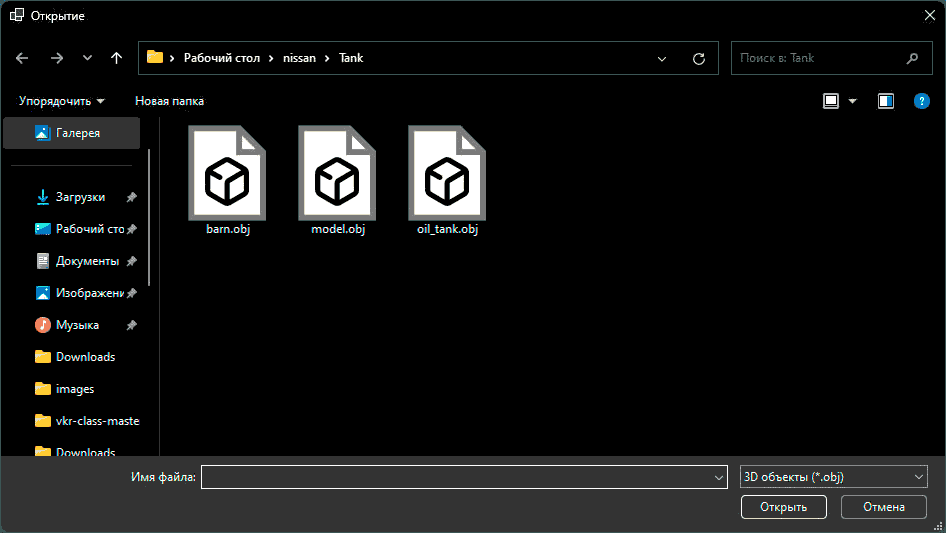
\includegraphics[width=0.75\linewidth]{screen6.png}}
	\caption{Диалоговое окно выбора файла}
	\label{screen6:image}
\end{figure}

В данном окне пользователь выбирает желаемый файл трёхмерной модели и нажимает на кнопку "<Открыть">. Если данный файл уже был загружен в проект, то на экране появится диалоговое окно, информирующее пользователя о перезаписи существующего файла. После окончания загрузки файла в проект, то появится диалоговое окно, информирующее пользователя об успешном импорте файла в проект (рисунок ~\ref{screen7:image}).

\begin{figure}[H]
	\center{
\includegraphics[width=0.75\linewidth]{screen7.png}}
	\caption{Диалоговое окно успешного импорта файла}
	\label{screen7:image}
\end{figure}

После загрузки файла, необходимо проверить корректно ли прошёл импорт. Пользователь переходит во вкладку "<Объект"> и нажимает на строку выпадающего списка того же типа, которого и был раннее загружен файл в проект. Так как пользователь загружал модель, то и нажмёт он на список, содержащий трёхмерные модели в проекте. Результат показан на рисунке ~\ref{screen8:image}.

\begin{figure}[H]
	\center{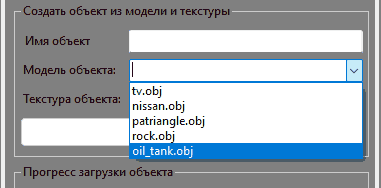
\includegraphics[width=0.8\linewidth]{screen8.png}}
	\caption{Список загруженных моделей в проект}
	\label{screen8:image}
\end{figure}

Как видно на снимке экрана, в конец выпадающего списка моделей добавилась новая позиция с наименованием файла модели oil\_tank.obj, который и загрузил пользователь немного раннее.

\subsubsection{Тестовый случай: Удаление ресурсов из проекта}
Действия пользователя: Пользователь выполняет действия для удаления соответствующего ресурса из проекта.

Ожидаемый результат: Файлы ресурсов, их ассоциации и объекты, связанные с данными ресурсами будут удалены из проекта, без возможности дальнейшего взаимодействия с ними.

Ход выполнения:

В открытой программе пользователь, переключившись на окно Инспектора, переходит во вкладку "<Модели и текстуры">.

На активном окне вкладки "<Модели и текстуры"> пользователю предоставляются списки моделей и текстур, находящиеся в проекте. В данных списках пользователь выбирает желаемый ресурс для удаления, нажав на его имя. После того, как желаемый ресурс будет выделен, пользователь нажимает на кнопку "<Удалить модель">. На экране высвечивается сообщение об успешном удалении модели из проекта. 

Но в случаях, когда данная модель являлась составляющей какого-либо существующего объекта в программе, то пользователю будет высвечено сообщение со списком объектов, которые были уничтожены, в связи с удалением их трёхмерной модели из проекта, как показано на рисунке ~\ref{screen9:image}.

\begin{figure}[H]
	\center{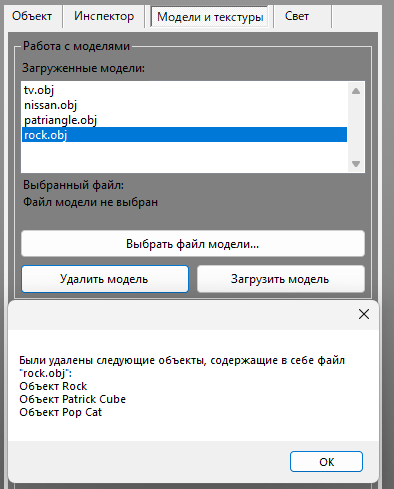
\includegraphics[width=0.8\linewidth]{screen9.png}}
	\caption{Вывод сообщения со списком удаленных объектов в проекте}
	\label{screen9:image}
\end{figure}

Перейдя во вкладку "<Объект">, и открыв выпадающий список моделей, можно увидеть на рисунке ~\ref{screen10:image}, что модель удаленного файла, также была удалена из списка прогружаемых моделей в проекте.

Далее, открыв выпадающий список объектов, можно увидеть на рисунке ~\ref{screen11:image}, что объекты, содержащие удаленную модель, также были удалены из проекта.

\begin{figure}[H]
	\center{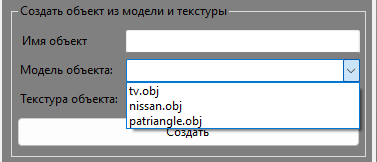
\includegraphics[width=0.8\linewidth]{screen10.png}}
	\caption{Список, демонстрирующий оставшиеся модели проекта, после удаления файла rock.obj}
	\label{screen10:image}
\end{figure}

\begin{figure}[H]
	\center{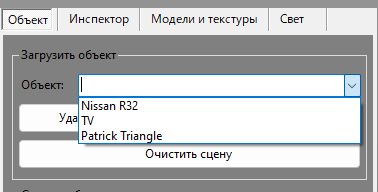
\includegraphics[width=0.8\linewidth]{screen11.png}}
	\caption{Список, демонстрирующий оставшиеся объекты в проекте, после удаления файла rock.obj}
	\label{screen11:image}
\end{figure}

\subsubsection{Тестовый случай: Создание нового объекта}
Действия пользователя: Пользователь создаёт новый объект, введя его имя и выбрав модель с текстурой.

Ожидаемый результат: В проекте создаётся новый объект, с указанным пользователем названием.

Ход работы:

В открывшемся окне инспектора, пользователь вводит желаемое имя для объекта напротив надписи "<Имя объекта">, а также выбирает модель и текстуру для данного объекта из выпадающих списков чуть ниже. Корректное и полное заполнение полей для создания объекта показано на рисунке ~\ref{screen12:image}.

\begin{figure}[H]
	\center{
\includegraphics[width=0.8\linewidth]{screen12.png}}
	\caption{Пример корректного заполнения полей для создания нового объекта}
	\label{screen12:image}
\end{figure}

Нажав на кнопку "<Создать">, система уведомит об успешном создании объекта с указанным именем.

Теперь пользователь может загрузить на сцену только что созданный объект. На той же вкладке, открыв выпадающий список объектов, в его конце появится имя нового объекта (рисунок ~\ref{screen13:image}).

\begin{figure}[H]
	\center{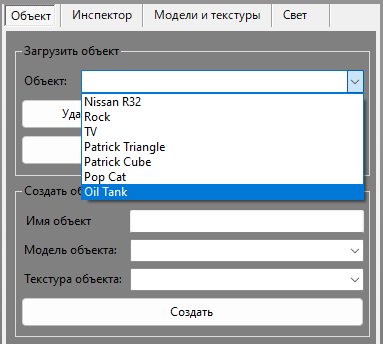
\includegraphics[width=0.8\linewidth]{screen13.png}}
	\caption{Обновленный список объектов, в который был добавлен объект Oil Tank}
	\label{screen13:image}
\end{figure}

После того, как в проект был добавлен объект с указанным именем и связанными с ним моделью и текстурой, можно проверить корректность его отображения на виртуальной сцене. Выбрав имя объекта в выпадающем списке, и нажав на кнопку "<Загрузить">, в главном окне программы будет отрисован текущий объект. Результат визуализации нового объекта показан на рисунке ~\ref{screen14:image}.

\begin{figure}[H]
	\center{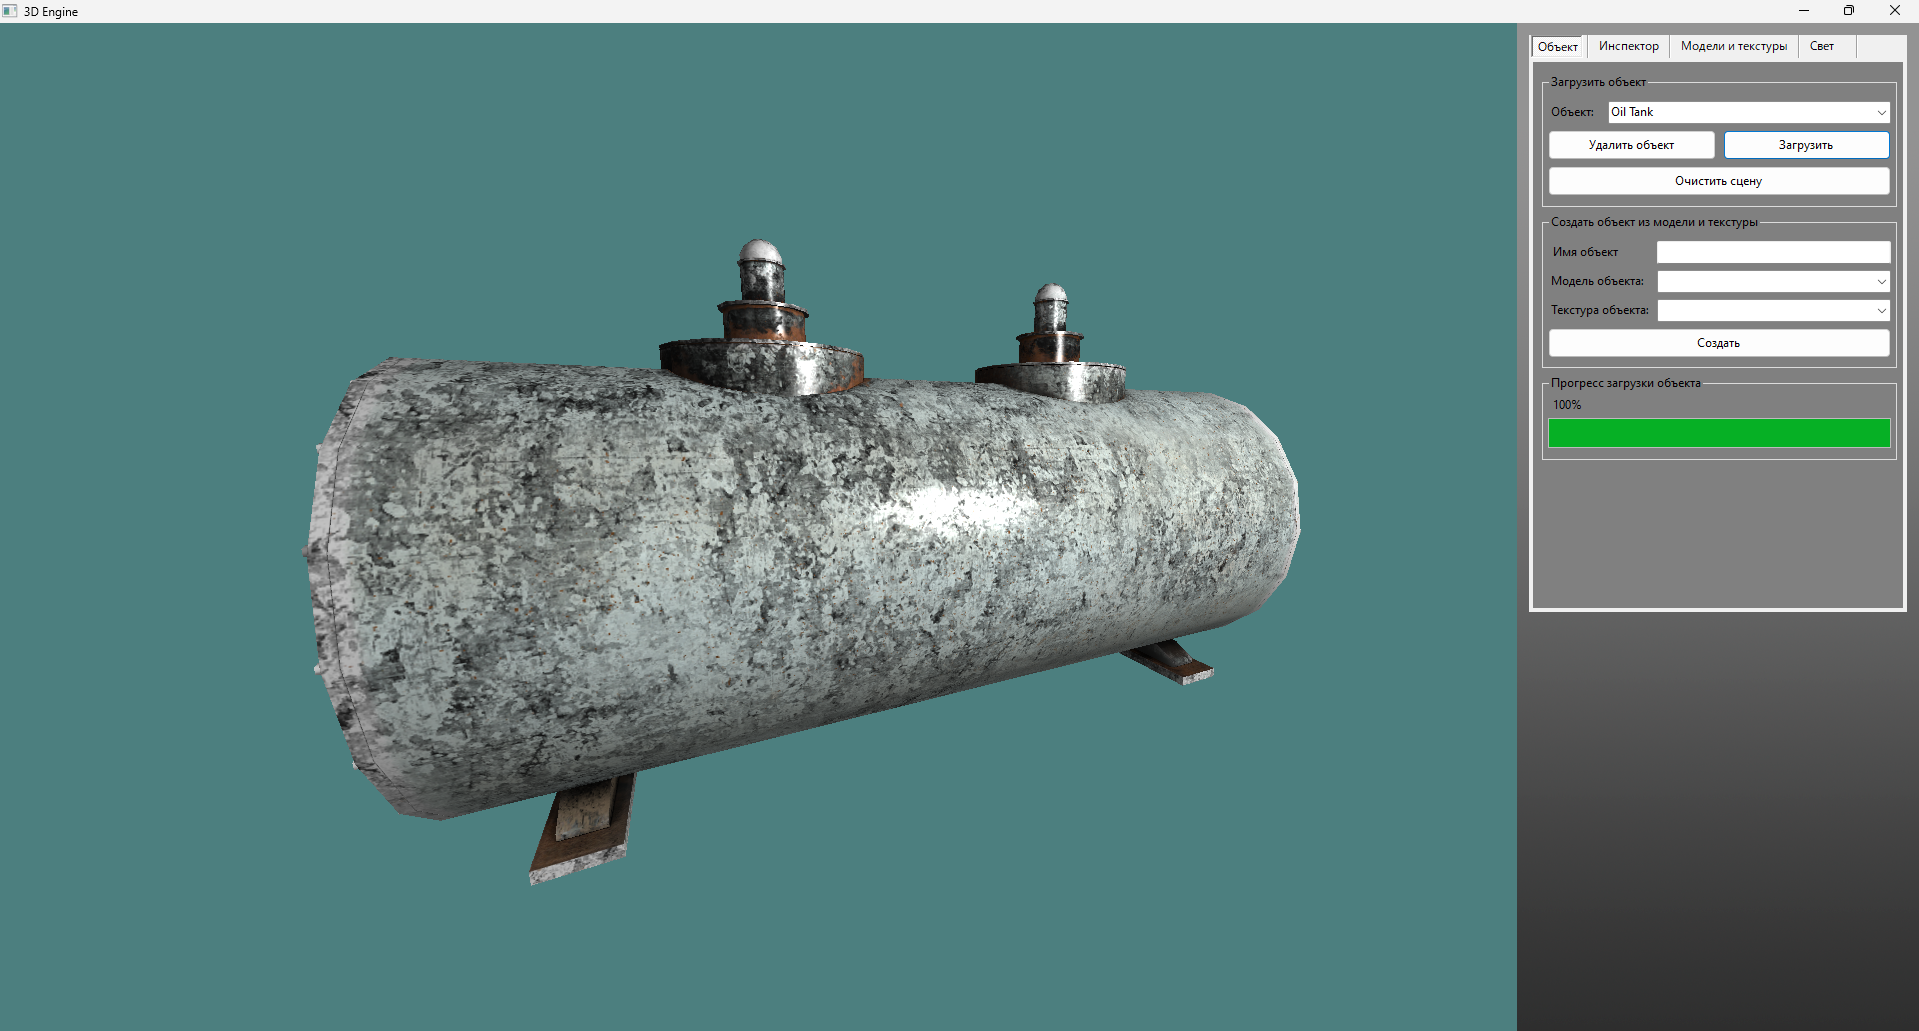
\includegraphics[width=1\linewidth]{screen14.png}}
	\caption{Результат визуализации объекта на сцене, созданного пользователем}
	\label{screen14:image}
\end{figure}

На данном снимке экрана можно увидеть, что модель и текстура объекта на виртуальной сцене отображена корректно.
   \section*{ЗАКЛЮЧЕНИЕ}
\addcontentsline{toc}{section}{ЗАКЛЮЧЕНИЕ}

Задача трехмерной графики — презентовать объект, явление или пространство в стилизованной или реалистичной визуальной форме. Дизайнеры рисуют предметы почти с нуля, настраивают освещение, работают над композицией кадра и в целом выполняют большую работу, поэтому с каждым годом трёхмерная компьютерная графика становится реалистичнее.

Постоянное совершенствование компьютерного оборудования и программного обеспечения сделало 3D-технологии доступными. Сегодня 3D-модели повсеместно используют вместо обычных макетов в проектировании для проработки крупных или миниатюрных деталей, а «объемная» визуализация становится одним из инструментов маркетинговых мероприятий, интерактивных тренингов, презентаций.

Основные результаты работы:

\begin{enumerate}
\item Проведен анализ предметной области. Выявлена необходимость использовать библиотеку OpenGL.
\item Разработана концептуальная модель программы. Разработана модель данных системы. Определены требования к системе.
\item Осуществлено проектирование программной системы. Разработана основа графического движка. Разработан пользовательский интерфейс приложения.
\item Реализована и протестирована программная система. Проведено системное тестирование.
\end{enumerate}

Все требования, объявленные в техническом задании, были полностью реализованы, все задачи, поставленные в начале разработки проекта, были также решены.

Готовый рабочий проект представлен в виде десктопного приложения. Приложение записано на внешний носитель информации, который приложен к отчёту.  
}\fi
\addcontentsline{toc}{section}{СПИСОК ИСПОЛЬЗОВАННЫХ ИСТОЧНИКОВ}

\begin{thebibliography}{13}

    \bibitem{opengl}	Дэвид Вольф: OpenGL 4. Язык шейдеров. Книга рецептов / Д. Вольф – Москва~: ДМК-Пресс, 2015. – 368 с. – ISBN 978-5-97060-255-3. – Текст~: непосредственный.
    \bibitem{opengl2}	C\# 8.0 и .NET Core 3.0 – Модернизация кросс-платформенной разработки / М. Дж. Прайс – Packt Publishing, 2019. – 818 с. – ISBN 978-1-78847-812-0. - Текст~: непосредственный.
    \bibitem{сsharpnew}	Компьютерная графика и 3D-моделирование: учебное пособие для СПО/  Л. Ю. Забелин, О. Л. Штейнбах, О. В. Диль / Профобразование, 2023. ISBN 978-5-4488-1594-2 - Текст~: непосредственный.
    \bibitem{22}	Обработка и визуализация пространственных данных на гибридном вычислительном кластере / В. А. Бобков, А. С. Черкашин - Синергия, 2014. - ISBN 978-5-04-015250-6. - Текст~: непосредственный.
    \bibitem{csharpopengl}	C\#. Программирование 2D и 3D векторной графики /Н. А. Тюкачев, В. Г. Хлебостроев – Санкт-Петербург~: Лань, 2022. – 320 с. – ISBN 978-5-8114-8988-6. – Текст~: непосредственный.
	\bibitem{html5}	Объектно-ориентированное программирование с примерами на C\#. Учебное пособие. Студентам ВУЗов. / П.Б. Хорев – Москва~: Форум, 2023. – 200 с. – ISBN 978-5-00091-680-3. – Текст~: непосредственный.
	\bibitem{htmlcss}	3D Graphics Rendering Cookbook / С. Косаревский, В. Латыпов – Packt Publishing, 2021. – ISBN 978-1-83898-619-3. - Текст~: непосредственный.
	\bibitem{bigbook}	OpenGL ES 3.0. Руководство разработчика / Д. Гинсбург – БХВ-Петербург, 2014. – ISBN 978-5-97060-256-0. - Текст~: непосредственный.
	\bibitem{uchiru}	Введение в трехмерную компьютерную графику с использованием библиотеки OpenGL / Ю. Кошкина, М. Персова - Новосибирский государственный технический университет, 2019. - ISBN 978-5-7782-3744-5. - Текст~: непосредственный.
	\bibitem{chaynik}	Программирование на C\# для начинающих. Особенности языка / А.Н. Васильев  – Москва : Бомбора, 2022. – 528 с. – ISBN 978-5-04-092520-9. – Текст~: непосредственный.
	\bibitem{1231}	Модели освещения и алгоритмы затенения в компьютерной графике / А. Г. Задорожный - Новосибирский государственный технический университет, 2023. - ISBN 978-5-7782-4308-8. - Текст~: непосредственный.
	\bibitem{sdf}	OpenGL ES 3.0. Руководство разработчика / Д. Гинсбург, Б. Пурномо - ДМК Пресс, 2014 - ISBN 978-5-97060-256-0. - Текст~: непосредственный.
	\bibitem{servsssds}	C\# 5.0. Карманный справочник / Д. Албахари, Б. Албахари - Диалектика-Вильямс, 2015 - ISBN 978-5-8459-1820-8. - Текст~: непосредственный.
\end{thebibliography}
\ifВКР{\appendix{Представление графического материала}

Графический материал, выполненный на отдельных листах,
изображен на рисунках А.1--А.\arabic{числоПлакатов}.
\setcounter{числоПлакатов}{0}

\renewcommand{\thefigure}{А.\arabic{figure}} % шаблон номера для плакатов

\begin{landscape}

\begin{плакат}
    
\includegraphics[width=0.82\linewidth]{plakat1.eps}
    \заголовок{Сведения о ВКРБ}
    \label{pl1:image}      
\end{плакат}

\begin{плакат}
    
\includegraphics[width=0.82\linewidth]{plakat2.eps}
    \заголовок{Цель и задачи разработки}
    \label{pl2:image}      
\end{плакат}

\begin{плакат}
    \includegraphics[width=0.82\linewidth]{plakat3.eps}
    \заголовок{Диаграмма конвеера данных}
    \label{pl3:image}      
\end{плакат}

\begin{плакат}
    \includegraphics[width=0.82\linewidth]{plakat4.eps}
    \заголовок{Диаграмма вариантов использования}
    \label{pl4:image}      
\end{плакат}

\begin{плакат}
	\includegraphics[width=0.82\linewidth]{plakat5.eps}
	\заголовок{Диаграмма классов программы}
	\label{pl5:image}      
\end{плакат}

\begin{плакат}
	\includegraphics[width=0.82\linewidth]{plakat6.eps}
	\заголовок{Прототип компонентов программы}
	\label{pl6:image}      
\end{плакат}

\begin{плакат}
	\includegraphics[width=0.82\linewidth]{plakat7.eps}
	\заголовок{Прототип интерфейса программы}
	\label{pl7:image}      
\end{плакат}

\begin{плакат}
	\includegraphics[width=0.82\linewidth]{plakat8.eps}
	\заголовок{Интерфейс программы}
	\label{pl8:image}      
\end{плакат}

\begin{плакат}
	\includegraphics[width=0.82\linewidth]{plakat9.eps}
	\заголовок{Результат визуализации трёхмерных данных}
	\label{pl9:image}      
\end{плакат}

\end{landscape}
}\fi
\ifПрактика{\appendix{Пример содержания OBJ-файла}

cube.obj
\lstinputlisting[language=Tex, frame=none]{cube.obj}

\appendix{Пример содержания файлов, описывающие хранимые ресурсы проекта}
Resources.data
\lstinputlisting[language=Tex, frame=none]{Resources.data}

Objects.data
\lstinputlisting[language=Tex, frame=none]{Objects.data}

\appendix{Листинг фрагмента программы парсера}
\lstinputlisting[language=Tex, frame=none]{parser_example.txt}

\ifВКР{
\newpage
\addcontentsline{toc}{section}{На отдельных листах (CD-RW в прикрепленном конверте)}
\begin{center}
\textbf{Место для диска}
\end{center}
}\fi}\else{\appendix{Пример содержания OBJ-файла}

cube.obj
\lstinputlisting[language=Tex, frame=none]{cube.obj}

\appendix{Пример содержания файлов, описывающие хранимые ресурсы проекта}
Resources.data
\lstinputlisting[language=Tex, frame=none]{Resources.data}

Objects.data
\lstinputlisting[language=Tex, frame=none]{Objects.data}

\appendix{Листинг фрагмента программы парсера}
\lstinputlisting[language=Tex, frame=none]{parser_example.txt}

\ifВКР{
\newpage
\addcontentsline{toc}{section}{На отдельных листах (CD-RW в прикрепленном конверте)}
\begin{center}
\textbf{Место для диска}
\end{center}
}\fi}\fi
\end{document}
